Você precisa entender os conceitos de orientação a objetos, OO, antes de aplicá-los com sucesso no desenvolvimento de sistemas. Como as técnicas OO emergiram, em parte, de áreas da engenharia de software, da inteligência artificial e da modelagem da informação, muitas dessas técnicas podem parecer já familiares para quem já trabalha na área de desenvolvimento de software. Não permita que esta familiaridade o torne complacente -- você ainda terá vários conceitos novos para aprender.

% texto sobre os paradigmas de programação
Antes de começar com a orientação a objetos, relembre os principais paradigmas de programação disponíveis para o desenvolvimento de software.
\begin{itemize}
\item Programação imperativa
\item Programação estruturada
\item Programação funcional
\item Programação orientada a objetos
\item Programação por prototipagem
\item Programação por aspectos
\end{itemize}

Estes paradigmas, estilos de programação, são todos equivalentes no sentido em que todos devem permitir a resolução dos mesmos problemas com um computador, uma máquina de Turing. A diferença está na facilidade de exprimir conceitos computacionais abstratos usados para a resolução dos problemas.

Estes diferentes paradigmas são apropriados para resolver diferentes tipos de problemas e desenvolvimentos. A programação imperativa, tão criticada por muitos desenvolvedores, pode ser útil no desenvolvimento de pequenas aplicações e bibliotecas que precisem de alto desempenho. Atualmente, a programação funcional voltou a receber uma grande atenção. A programação com JavaScript chama a atenção para a programação por prototipagem. Algumas linguagens de programação dão suporte a um ou vários paradigmas. A orientação a objetos é um dos principais paradigmas para a reutilização de código.

Os programadores novatos, muitas vezes, se desencorajam com a burocracia da programação orientada a objetos. Isto se deve principalmente à baixa complexidade dos problemas que lhes são propostos para resolver. Os novatos não entendem a vantagem de descobrir erros na compilação em vez de encontrá-los na execução. A resolução de problemas simples geralmente se beneficiam do uso de bibliotecas, especialmente as de entradas e saídas de dados, mas não há a necessidade de criar suas próprias bibliotecas (onde está o reuso de código). A orientação a objetos é muito importante para o projeto e implementação de soluções para problemas mais complexos. A orientação a objetos permite modelar melhor o domínio do problema, do sistema e da solução. O que resulta em uma decomposição mais natural do código e um melhor reuso dele. Um aspecto extremo deste reuso é a aplicação de padrões de projeto, \textit{design patterns}, onde percebe-se que determinados problemas, não só de computação, são encontrados e reencontrados com frequência. No lugar de tentar reinventar uma solução, pode-se reutilizar uma solução já estada e aprovada. A análise e modelagem deste tipo de euso, muitas vezes, usa a modelagem OO.

Um outro diferencial da programação orientada a objetos é o tratamento de erros. Na programação OO, a estrutura \emph{try-catch} permite isolar o código para o processamento sem erros do código para o processamento das situações com erro. Na programação imperativa usual, este tratamento é feito com o uso de estruturas condicionais que tornam a legibilidade e manutenção do código bastante complexa.

A seguir veremos:

\begin{itemize}
\item Uma rápida introdução aos conceitos de OO;
\item Conceitos OO do ponto de vista estruturado;
\item Os diagramas da linguagem unificada de modelagem (UML 2);
\item Objetos e classes;
\item Atributos e operações;
\item Abstração, encapsulamento e ocultação de informação (\textit{information hiding});
\item Herança;
\item Persistência;
\item Relacionamentos;
\item Colaboração;
\item Polimorfismo;
\item Interfaces;
\item Componentes; e
\item Padrões.
\end{itemize}

\section{Uma rápida introdução aos conceitos de OO}

Nesta seção são vistos alguns conceitos fundamentais das técnicas de desenvolvimento OO. Programadores experientes com tecnologias estruturadas já conhecem muitos destes conceitos, outros, porém, são novos. Por exemplo, os conceitos que estão no núcleo de OO como encapsulamento, acoplamento e coesão vêm da engenharia de software. Estes conceitos são importantes porque eles revelam boas práticas de projeto independentemente da tecnologia que está sendo usada. Não se engane, entretanto, não é porque você já viu alguns dos conceitos e os pratica que você já está fazendo OO, mas você já está realizando bons projetos. Enquanto fazer bons projetos é uma grande parte da orientação a objetos, ainda há muito mais.

Os conceitos de OO parecem muito simples. Mas, os conceito em que se baseiam as técnicas estruturadas também pareciam simples, os programadores experientes sabem que o desenvolvimento estruturado é na verdade difícil. Assim como havia mais do que uns poucos conceitos simples no paradigma estruturado, há mais coisas no paradigma OO do que os conceitos básicos que veremos. Assim como leva tempo para se tornar um bom desenvolvedor estruturado, também leva tempo para se tornar um bom desenvolvedor OO. Dentre os diversos paradigmas de programação, o que pode parecer mais simples é o da programação funcional, pois nele usamos basicamente funções recursivas para obter iterações e composição de funções para obter funções mais complexas. É, entretanto, longe de ser simples a resolução de problemas complexos com a programação funcional. Para lhe dar um gostinho do conteúdo deste texto, alguns dos principais conceitos e termos que serão apresentados são resumidos na tabela \ref{tab:concOO}.

\begin{longtable}[l]{p{4.6cm}p{11.1cm}}
\caption[Conceitos OO]{\bfseries Conceitos e termos da Orientação a Objetos}
\label{tab:concOO}\\

\multicolumn{1}{c}{\textbf{Termo}} & \multicolumn{1}{c}{\textbf{Descrição}} \\
\midrule
\endfirsthead

\multicolumn{2}{c}{{\bfseries \tablename\ \thetable{} -- continuação da página anterior}} \\
\multicolumn{1}{c}{\textbf{Termo}} & \multicolumn{1}{c}{\textbf{Descrição}} \\
\midrule
\endhead

\multicolumn{2}{r}{{Continua na próxima página}} \\% \hline
\endfoot

\hline %\hline

\endlastfoot

Abstração & As características essenciais de um item (pode ser uma classe ou uma operação) \\

Acoplamento & O grau de dependência entre dois itens\\

Agregação & Relacionamento entre duas classes ou componentes definidas por \emph{é parte de}\\

Hierárquia de agregação & Um conjunto de classes relacionadas através da agregação\\

Associação & Um relacionamento entre duas classes ou objetos\\

Atributo & Algo que uma classe conhece (dados/informação)\\

Cardinalidade & O conceito de \emph{quantos?}\\

Classe & Uma abstração em software de objetos similares, um padrão a partir do qual objetos são criados\\

Classe abstrata & Uma classe que não pode ter objetos instanciados dela \\

Classe concreta & Uma classe que pode ter objetos instanciados dela\\

Classificador & Um termo de UML para uma coleção de instâncias que têm algo em comum. Isto inclui classes, componentes, tipos de dados e casos de uso\\

Coesão & O grau de relacionamento de uma unidade encapsulada (tal como um componente ou uma classe)\\

Colaboração & Classes que trabalham juntas (colaboram) para cumprir as suas responsabilidades\\

Componente & Uma unidade coesa de funcionalidade que pode ser desenvolvida, entregue e composta por outros componentes para construir uma unidade maior\\

Composição & Uma forma forte de agregação na qual o \emph{todo} é completamente responsável pelas suas partes e cada objeto \emph{parte} está associado apenas a um objeto \emph{completo}\\

Encapsulamento & O agrupamento de conceitos relacionados num único item, tal como uma classe ou um componente\\

Estereótipo & Um uso comum de um elemento de modelagem\\

Herança & Relacionamento definido por \emph{é um} ou \emph{é como} (ou \emph{parece com})\\

Herança múltipla & A herança direta de mais de uma classe\\

Herança simples & A herança direta de apenas uma classe\\

Hierárquia de heranças & Um conjunto de classes relacionadas por heranças\\

Instância & Um objeto que é um exemplo de uma classe específica\\

Instanciar & Criar objetos a partir da definição de classes\\

Interface & Uma coleção de uma ou mais assinaturas de operações que define um conjunto coeso de comportamentos\\

Mensagem & Um pedido por informação ou para realizar uma ação\\

Mensageria (ou caixa postal) & Um processo de colaboração entre objetos pelo envio de mensagens uns para os outros\\

Método & Um processo implementado por uma classe que realiza uma ação de valor (similar a uma função na programação estruturada)\\

Objeto & Uma pessoa, lugar, coisa, evento, conceito, tela ou relatório baseado numa definição de classe\\

Objeto persistente & Um objeto salvo numa memória permanente\\

Objeto transitório & Um objeto não salvo numa memória permanente\\

Ocultação de informação & A restrição ao acesso externo de atributos\\

Opcionalidade & O conceito de \emph{Você precisa ter isto?}\\

Padrão de projeto & Uma solução reusável para um problema comum levando em conta forças relevantes\\

Persistência & O armazenamento de objetos em memória permanente, por exemplo, em arquivos, bancos de dados, etc.\\

Perspectivas & Os objetos podem ser vistos sob três perspectivas: Do conceito, da especificação e da implementação \\

Polimorfismo & A capacidade de diferentes objetos responderem a uma mesma mensagem de maneiras diferentes, permite que um objeto interaja com um outro sem conhecer o seu tipo exato\\

Propriedade & Em UML 2, um valor nomeado (com nome), por exemplo, atributos e associações, inclusive composição, denotando uma característica de um elemento (tal como, uma classe, ou um componente). Em C\#, a combinação de um atributo com seus getter e setter \\

Refatoração & Modificar a implementação e/ou a definição de componentes sem afetar outros componentes de um sistema já em funcionamento\\

Sobreescrita & Redefinir atributos e/ou métodos em subclasses tais que eles sejam diferentes da definição na superclasse\\

Subclassse & Uma classe que herda de uma outra\\

Superclase & Uma classe da qual uma outra herda.\\

\end{longtable}
\noindent {Fonte: Fortemente baseada em \cite{Ambler:TOP:3ed}}
 
\section{Conceitos de OO do ponto de vista estrutural}

Provavelmente, você se assustou com a lista de conceitos da Tabela \ref{tab:concOO}. Se você está estudando para um teste, supõe-se que a lista seja útil para você. A maioria de nós procura por uma maneira de aprender os conceitos OO facilmente. Antes de ver as explicações detalhadas, vamos descrever quatro conceitos básicos de OO rapidamente, numa linguagem que pode ser familiar para você, a terminologia estruturada.

\begin{description}
\item[Classe] Uma classe é uma abstração de software de um objeto, efetivamente, um padrão a partir do qual os objetos são criados. Se você tiver experiência com bancos de dados, você pode pensar numa classe como uma tabela, embora tenha mais em classes do que isto conforme você verá mais tarde. A definição de uma classe descreve o layout, incluindo tanto os dados, quanto as funcionalidades, dos objetos a serem criados a partir deles. Observe que eu disse, tanto os dados, quanto as funcionalidades. Diferente de uma tabela, que define apenas dados, uma classe define ambos, dados (atributos) e código (operações/métodos). Por enquanto, uma boa maneira de pensar a respeito de uma classe é que ela é a combinação de uma definição de tabela e a definição do código fonte que acessa os dados. Infelizmente, esta é uma visão muito orientada a dados de objetos que ignora a principal força dos objetos que é a capacidade de responder a pedidos de ações.

\item[Objeto] Um objeto é uma construção de software que espelha um conceito do mundo real, por exemplo, uma pessoa, lugar, coisa, evento, conceito, tela ou relatório. Objetos são tipicamente (mas nem sempre) nomes próprios, substantivos. Se uma classe pode ser pensada como uma tabela, um objeto pode ser pensada como a ocorrência de um registro. De novo, esta é uma visão muito orientada a dados. Por exemplo, um objeto estudante pode fazer muitas das coisas que um estudante \emph{real} pode, por exemplo, fornecer seu nome, calcular quantos anos tem e requerer a inscrição numa disciplina. Numa aplicação estruturada, cada estudante seria representado como um registro na tabela de dados Estudante. Numa aplicação orientada a objetos, cada estudante seria representado por um objeto na memória. A principal diferença é que onde registros de estudantes só têm dados, os objetos estudantes têm ambos, dados (atributos) e funcionalidades (métodos). Do ponto de vista de projeto, é conveniente entender os objetos como entidades com responsabilidades, estas responsabilidades incluem as informações que o objeto detem e as ações que ele pode realizar.

\item[Atributo] Um atributo é equivalente a um elemento de dados num registro. Do ponto de vista de programação, também faz sentido pensar num atributo como uma variável local aplicável a apenas um objeto. Os objetos são responsáveis pelas suas próprias informações que devem ser guardadas nos atributos dos objetos. Existem informações que não são de responsabilidade dos objetos individualmente, mas de todos os objetos de um mesmo tipo/classe, nesse caso, temos atributos de classe. Quando cada objeto, chamado de instância de uma classe, tem seu próprio atributo, este atributo é chamado de atributo de instância.

\item[Método] Um método pode ser pensado tanto como uma função ou um procedimento. Métodos acessam e modificam os atributos de um objeto. Melhor ainda, métodos podem fazer toda uma série de coisas que nada têm a ver com os atributos. Alguns métodos retornam um valor (como as funções), enquanto outros provocam efeitos colaterais, como impressão ou armazenamento em memória permanente, ou mudam o valor de um atributo, dizemos que o método muda o estado do objeto, ou de outro objeto associado. Um método útil deve ou retornar um valor, ou ter um efeito colateral significativo. Em terminologia OO, dizemos que os objetos trocam mensagens entre eles. Uma mensagem de um objeto para um outro requer uma ação de responsabilidade deste último. A maneira de ``enviar'' a mensagem é o primeiro objeto chamar o método do segundo objeto. Este é o modelo da maioria das linguagens de programação para aplicações locais. Em sistemas distribuidos, é possivel que a chamada de um método efetivamente provoque o envio de uma mensagem de um objeto local para um objeto remoto.

\end{description}

Atributos e métodos de uma classe são chamados de membros de uma classe de forma geral. Algumas características se aplicam tanto a atributos, quanto a métodos, por isso o conceito de membro da classe é útil.

\cite{uml:destilado} descreve três perspectivas diferentes no processo de desenvolvimento OO que ajudam a determinar as classes:

\begin{description}
\item[Perspectiva Conceitual] Esta perspectiva ``representa os conceitos do domínio estudado ... um modelo conceitual deve ser obtido sem, ou com pouca, ligação com o software que vai implementá-lo ...'' Ela responde à pergunta: ``\emph{Pelo que sou responsável?}''

\item[Perspectiva da Especificação] ``Agora olhamos para o software, não para a implementação, mas para as interfaces.'' Ela responde à pergunta: ``\emph{Como sou usado?}''

\item[Perspectiva da Implementação] Estamos na visão do próprio código. ``Esta é provavelmente a perspectiva mais usada, mas de muitas maneiras, a perspectiva da especificação é melhor.'' Ela responde à pergunta: ``\emph{Como cumpro minhas responsabilidades?}''
\end{description}

\cite{DP:explained} afirma que a melhor maneira de projetar as classes é pela determinação das suas responsabilidades. O projeto de software antigamente usava basicamente a perspectiva de implementação que é mais próxima aos programadores, mas os projetos resultantes são pouco flexíveis e difíceis de serem mantidos. Em software, os requisitos dos projetos mudam com frequência, esta maneira de projetar não se adapta bem às mudanças nos requisitos. É melhor projetar pela perspectiva da especificação, pelas interfaces. Esta perspectiva resulta em projetos mais adaptáveis às mudanças de requisitos. Os padrões de projeto também usam esta maneira de especificar as soluções. \cite{design:patterns} usa com frequência classes abstratas nos seus esquemas de soluções.

\section{Os diagramas de UML 2}

A \textit{Unified Modeling Language}, UML, é uma linguagem visual (isto é, ela é uma notação gráfica de diagramas com semântica) usada para criar modelos de programas. Neste contexto, o termo \textit{modelos de programas} significa representações em diagramas dos programas que mostram os relacionamentos entre os objetos no código. A tabela \ref{tab:useUML} ilustra o uso dos diagramas UML em diferentes momentos do desenvolvimento OO.

\begin{longtable}[l]{p{4.9cm}p{11cm}}
\caption{Os Diagramas de UML 2 e seus propósitos} \label{tab:useUML}\\

\multicolumn{1}{c}{\textbf{Quando você está}} & \multicolumn{1}{c}{\textbf{Diagramas UML a usar}} \\
\midrule
\endfirsthead

\multicolumn{2}{c}{{\bfseries \tablename\ \thetable{} -- continuação da página anterior}} \\
\multicolumn{1}{c}{\textbf{Quando você está}} & \multicolumn{1}{c}{\textbf{Diagramas UML a usar}} \\
\midrule
\endhead

\multicolumn{2}{r}{{Continua na próxima página}} \\% \hline
\endfoot

\hline %\hline
\endlastfoot

Na fase de análise & Diagramas de Caso de Uso, que envolvem entidades interagindo com o sistema (usuários e outros sistemas) e os pontos de função que você precisa implementar.\\

 & Diagramas de Atividade, cujo foco é o fluxo de trabalho do domínio do problema (o verdadeiro espaço onde as pessoas e outros agentes estão trabalhando, a área de trabalho do programa) e não o fluxo da lógica do programa.\\[0.3cm]
 
Na observação das interações dos objetos & Diagramas de Interação, que mostram como os objetos interagem entre eles. Por lidar com casos específicos e não com situações gerais, eles demonstram serem úteis tanto para verificar os requerimentos, quanto para verificar os projetos. O diagrama de interação mais popular é o Diagrama de Sequência. \\[0.3cm]

Na fase de projeto & Diagramas de Classe, que detalham os relacionamentos entre as classes.\\[0.3cm]

Na observação das mudanças de \textit{comportamento} em função do estado atual do objeto & Diagramas de Máquina de Estado, que detalha os diferentes estados em que o objeto pode estar e suas transições.\\[0.6cm]

Na fase de distribuição & Diagramas de Distribuição, que mostram como módulos diferentes serão distribuidos.

\end{longtable}
\noindent {Fonte: \cite{DP:explained}}\\

Entender os 14 diagramas de UML 2 ilustrados na figura \ref{fig:uml14dia} e resumidos na tabela \ref{tab:diaUML} é importante para a compreensão da análise e do desenvolvimento OO. Existem 3 classificações para os diagramas UML\footnote{Os diagramas UML 2 deste trabalho foram feitos usando a ferramenta Dia, \cite{dia:tool}.}:

\begin{description}
\item[\emph{Diagramas de Comportamento}:] Este é o tipo de diagrama que representa características comportamentais de um sistema ou processo de negócio. Isto inclui diagramas de atividade, máquina de estado e caso de uso, assim como os 4 diagramas de interação.

\item[\emph{Diagrams de Interação}:] Este é um subconjunto de diagramas comportamentais que enfatizam a interação entre objetos. Isto inclui os diagramas de comunicação, visão simplificada de interação, sequência e temporização.

\item[\emph{Diagramas Estruturais}:] Este tipo de diagrama representa os elementos estáticos de uma especificação que não mudam com o tempo. Isto inclui os diagramas de classe, estrutura composta, componente, distribuição (\textit{deployment}), objetos, pacotes e perfil.
\end{description}

\begin{figure}[h]
\begin{center}
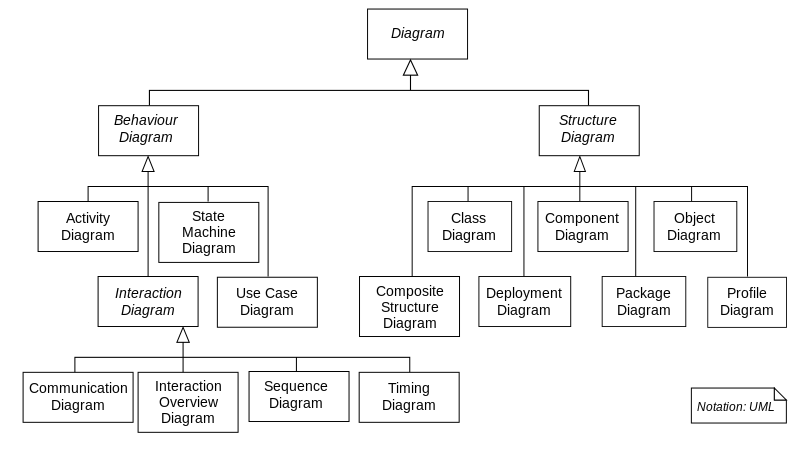
\includegraphics[scale=0.55]{UML_diagrams_overview.png} 
\caption{Hierárquia dos diagramas UML} \label{fig:uml14dia}
\end{center}
\legend{Fonte: \cite{wiki:uml}}
\end{figure}

\begin{longtable}[l]{p{4.7cm}p{11cm}}
\caption[Diagramas UML]{Os Diagramas de UML 2} \label{tab:diaUML}\\

\multicolumn{1}{c}{\textbf{Diagrama}} & \multicolumn{1}{c}{\textbf{Descrição}} \\
\midrule
\endfirsthead

\multicolumn{2}{c}{{\bfseries \tablename\ \thetable{} -- continuação da página anterior}} \\
\multicolumn{1}{c}{\textbf{Diagrama}} & \multicolumn{1}{c}{\textbf{Descrição}} \\
\midrule
\endhead

\multicolumn{2}{r}{{Continua na próxima página}} \\% \hline
\endfoot

\hline %\hline
\endlastfoot

Diagrama de Atividade & Representação de alto nível de processos de negócios, incluindo fluxos de dados ou modelagem da lógica complexa dentro de um sistema \\

Diagrama de Caso de  Uso & Mostra casos de uso, atores e seus relacionamentos \\

Diagrama de Classe & Mostra uma coleção de elementos de modelagem estáticos tais como classes e tipos, seus conteúdos e seus relacionamentos \\

Diagrama de Componente & Representa os componentes, inclusive seus interrelacionamentos e interfaces públicas, que compõem uma aplicação, sistema ou empresa \\

Diagrama de Comunicação & Mostra instâncias de classes, seus interrelacionamentos e o fluxo de mensagens entre elas e tipicamente foca na organização estrutural de objetos que enviam e recebem mensagens; eram chamados de diagramas de colaboração no UML 1 \\

Diagrama de Distribuição & Mostra a arquitetura de execução dos sistemas, inclusive os nós, tanto os ambientes de execução de HW, quanto de SW, e o \textit{middleware} que os conecta \\

Diagrama de Estrutura Composta & Representa a estrutura interna de um classificador (tal como uma classe, componente ou caso de uso), inclusive os pontos de interação do classificador com outras partes do sistema \\

Diagrama de Máquina de Estado & Descreve os estados em que um objeto ou uma interação podem estar, assim como as transições entre os estados. Anteriormente, era chamado de diagrama de estados, diagrama do mapa de estados ou diagrama de transição de estados  \\

Diagrama de Objetos & Representa objetos e seus relacionamentos num instante determinado, tipicamente, um caso especial de um diagrama de classes ou de comunicação \\

Diagrama de Pacotes & Mostra como elementos de modelagem são organizados em pacotes, assim como as dependências entre os pacotes \\

Diagrama de Perfil & Opera no nível do metamodelo para mostrar estereótipos como classes com o estereótipo «stereotype» e perfis como pacotes com o estereótipo «profile». A relação de extensão (linha sólida com ponta de seta fechada e preenchida) indica qual elemento metamodelo um determinado estereótipo está estendendo. Este diagrama não existia na UML 1 \\

Diagrama de Sequência & Modela a lógica sequencial, na verdade, a ordenação temporal das mensagens entre classificadores \\

Diagrama Simplificado de Interação & Uma variação do diagrama de atividade, que resume o fluxo de controle dentro de um sistema ou de um processo de negócios, onde cada nó/atividade no diagrama pode representar um outro diagrama de interação \\

Diagrama de Temporização & Representa a mudança de estado ou condição de uma instância, de um classificador ou de um papel (\textit{role}) ao longo do tempo. Tipicamente, usado para mostrar a mudança de estado de um objeto no tempo ao responder a um evento externo. \\

\end{longtable}
\noindent {Fonte: \cite{Ambler:TOP:3ed}}

\section{Objetos e Classes}

O paradigma OO é baseado em construir sistemas a partir de itens chamados de \emph{objetos}. Um objeto é uma pessoa, lugar, coisa, conceito, tela ou relatório. Uma classe generaliza/representa uma coleção de objetos similares e é efetivamente um padrão a partir do qual cria-se objetos. Num sistema universitário, Clara é um objeto estudante, ela está matriculada em diversos objetos disciplinas e ela trabalha para obter um objeto diploma de um objeto curso. Num sistema bancário, Clara é um objeto cliente. Ela tem um objeto conta para o qual ela pode preencher objetos cheques. Num sistema de controle de inventário, cada item do inventário é um objeto, cada entrega é um objeto e cada cliente é um objeto.

No mundo real, você tem objetos, logo, você precisa deles como um conceito para refletir precisamente o espaço do seu problema. Entretanto, no mundo real, objetos são frequentemente similares a outros objetos. Estudantes compartilham qualidades similares (eles fazem as mesmas coisas, eles são descritos da mesma forma), disciplinas compartilham qualidades semelhantes, itens de  inventórios, contas bancárias, ... compartilham qualidades semelhantes entre eles. Enquanto você pode modelar (e programar) todos os objetos individualmente, isto exige um trabalho enorme. É preferível definir o que é ser um estudante uma vez, definir disciplina uma vez, definir item de inventório uma vez, ... É por isso que você precisa do conceito de classe. Os objetos são exemplos/instâncias da classe.

\begin{figure}[h]
\begin{center}
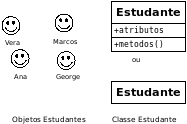
\includegraphics[scale=1]{objClassStdt.png} 
\caption[Objetos e Classe \emph{Estudante}]{Objetos \emph{Estudante} e duas maneiras de modelar a classe \emph{Estudante}} \label{fig:objStdt}
\end{center}
\end{figure}

A figura \ref{fig:objStdt} ilustra como temos objetos estudantes e como podemos modelar a classe \emph{Estudante}. Ela também mostra a notação padrão para modelar uma classe usando UML. Classes são tipicamente modeladas por uma das duas maneiras: um retângulo com uma lista dos atributos e métodos da classe ou apenas um retângulo. Existem razões para modelar classes de uma maneira ou da outra. Por um lado, listar os atributos e métodos pode ser bastante útil, permite aos leitores do modelo entender o projeto numa única visualização. Por outro lado, listar os atributos e métodos pode poluir seus diagramas e dificultar a leitura. Neste texto, serão usadas ambas as técnicas, os métodos e atributos só serão listados onde forem apropriados.

Nome de classe é tipicamente um substantivo no singular. O nome de uma classe pode ter uma ou duas palavras e deve descrever precisamente a classe usando terminologia comum ao domínio do negócio onde o problema está inserido. Se você tem dificuldades para dar nome a uma classe, ou você precisa entendê-la melhor, ou podem ser várias classes que você combinou erroneamente. Você deve modelar classes com nomes tais como \emph{Estudante}, \emph{Professor} e \emph{Disciplina} e não como \textit{Estudantes}, \textit{Pessoas que ensinam disciplinas} ou \textit{COMP101}. Pense da seguinte forma, no mundo real, você diria ``Sou um estudante'' e não ``Sou um estudantes''.

Classes também podem representar conceitos para os quais não existe um substantivo, como o processo de retirada de um livro de uma biblioteca.

Quando software OO está rodando, objetos são instanciados (criados/definidos) a partir de classes. Dizemos que um objeto é uma instância de uma classe e instanciamos estes objetos das classes.

Uma das maiores dificuldades no desenvolvimento de software OO é a escolha das classes que devem ser implementadas para resolver um problema. Um método mais antigo diz que devemos identificar os nomes (substantivos) do domínio do problema e as ações que  estes nomes executam para resolver o problema. Uma maneira mais atualizada de encontrar as classes é encontrar as responsabilidades para a solução do problema. No início da programação OO era comum encontrar classes que faziam muitas coisas, porque representavam objetos complexos, hoje, prefere-se classes pequenas que são responsáveis por um serviço, ou poucos serviços.

\section{Atributos e Operações/Métodos}

Classes têm responsabilidades, as coisas que elas sabem e fazem. Atributos são as coisas que as classes sabem, métodos são as coisas que elas fazem. O paradigma da orientação a objetos é baseado nos conceitos de que sistemas devem ser construídos a partir de objetos e estes objetos têm tanto dados, quanto funcionalidade. Atributos definem os dados, enquanto os métodos definem a funcionalidade.

Quando você define uma classe, você deve definir os atributos que ela tem, assim como, os seus métodos. Em UML 2, um atributo é um tipo de propriedade, como são relacionamentos tais como associação e composição. A definição de um atributo é direta. Você define seu nome, talvez seu tipo (se ele é um número, um string, uma data cronológica, etc.).  Linguagens fracamente tipadas como Smalltalk (ou Python) permitem que você use atributos da maneira que você quiser e, portanto, não exigem que você defina o tipo deles. Linguagens fortemente tipadas como Java e C++, entretanto, insistem que você defina o tipo de um atributo antes de você poder usá-lo. Você pode ainda escolher se você quer indicar alguma regra de negócio ou restrição aplicável ao atributo, tais como valores válidos que o atributo pode ter, vide figura \ref{fig:umlClsLmt}.

\begin{figure}[h]
\begin{center}
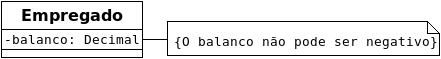
\includegraphics[scale=0.7]{umlClsLmt.png} 
\caption{Exemplo de classe com atributo limitado} \label{fig:umlClsLmt}
\end{center}
\end{figure}

A definição de um método é mais simples: você define a lógica para ele, do mesmo modo que você codifica uma função ou um procedimento. O termo \emph{método} é usado diferentemente de como a UML usa -- o que está sendo mostrado, na verdade, são as operações da classe e os métodos são as implementações dessas operações. Esta visão de método é consequência da influência do Smalltalk, que usa o termo método dessa maneira. Não se preocupe com isto, a terminologia de objetos é notoriamente inexata. Mais para a frente detalharemos melhor a especificação de métodos. Ao vermos o conceito de colaboração, você verá que colaboração é feita exclusivamente através de métodos. Por ora, retenha que métodos fazem estas duas coisas: eles retornam um valor e/ou eles fazem alguma coisa, isto é, eles provocam um efeito de borda. Em computação, efeito de borda (\emph{side effect}) significa que uma modificação é realizada por este método na memória e esta modificação é visível por outros métodos, isto é, fora deste método.

\begin{figure}
\begin{center}
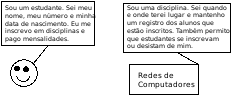
\includegraphics[scale=1]{obj2.png} 
\caption[Objetos no mundo real]{Objetos no mundo real} \label{fig:obj2}
\end{center}
\end{figure}

Na figura \ref{fig:obj2}, você vê dois tipos diferentes de objetos: um \textit{estudante} e uma \textit{disciplina}. Ambos objetos, sabem e fazem algumas coisas e você deseja registrar isto nos seus modelos, como você pode observar na figura \ref{fig:class1}. Estou usando a notação de classe com 3 seções neste caso: a seção do topo para o nome, a seção do meio para a lista dos atributos e a seção de baixo lista os métodos.

A figura \ref{fig:class1} expõe 2 tipos diferentes de atributos: atributos de instância que são aplicáveis a um único objeto e atributos estáticos que são aplicáveis a todas as instâncias de uma classe. Atributos estáticos têm o nome sublinhado, atributos de instância não são sublinhados. Por exemplo, \emph{nome} é um atributo de instância na classe Estudante. Cada estudante individual tem um nome, por exemplo, um estudante tem como nome ``José da Silva'', enquanto uma outra estudante pode ter o nome ``Maria de Oliveira''. Pode até acontecer de dois estudantes diferentes terem o mesmo nome, embora sejam duas pessoas diferentes.

\begin{figure}[h]
\begin{center}
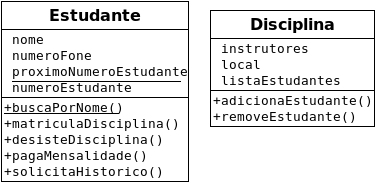
\includegraphics[scale=0.85]{class1.png} 
\caption{Classes \emph{Estudante} e \emph{Disciplina}} \label{fig:class1}
\end{center}
\end{figure}

Por outro lado, \emph{proximoNumeroEstudante} é um atributo estático (também chamado de atributo da classe) que é aplicável à classe Estudante, não especificamente a uma instância determinada. Este atributo é usado para guardar qual é o valor que será usado como número de estudante pelo próximo estudante a ser cadastrado. Quando um novo estudante ingressa na escola, seu número de estudante é dado pelo valor atual de \emph{proximoNumeroEstudante}, que será incrementado para garantir que o número de todos os estudantes é único.

De modo similar, existe o conceito de método de instância e método estático (ou de classe): Métodos de instância operam sobre uma única instância, enquanto métodos estáticos operam potencialmente sobre \textit{todas} as instâncias de uma classe\footnote{Um método estático não precisa de uma instância para operar, então ele pode ser executado mesmo se nenhuma instância ainda foi criada. Um cuidado que novatos devem ter, é que na implementação de um método de classe não é possível acessar atributos de instância.}. Na figura \ref{fig:class1}, observe que na classe \emph{Estudante} os métodos \emph{matriculaDisciplina()} e \emph{desisteDisciplina()} são métodos de instância, coisas que um estudante individual faria. Ela também tem um método estático \emph{buscaPorNome()}, que fornece o comportamento de procurar os estudantes cujo nome atendem um critério de busca, é um método que opera sobre todas as instâncias da classe.

\section{Abstração, Encapsulamento e Ocultação de Informação}

Em vez de dizer que determinamos o que uma classe \textit{sabe} e \textit{faz}, dizemos que \emph{abstraímos} a classe. Em vez de dizermos que projetamos como a classe realizará essas coisas, dizemos que \emph{encapsulamos} elas. Em vez de dizer que projetamos a classe restringindo o acesso aos seus atributos, dizemos que \emph{escondemos}, ocultamos, a informação.

\subsection{Abstração}

O mundo é um lugar complicado. Para lidar com esta complexidade, formamos abstrações das coisas dele. Por exemplo, considere a abstração de uma pessoa. Do ponto de vista da universidade, ela precisa saber o nome, endereço, número de telefone/celular, RG, CPF e formação acadêmica da pessoa. Do ponto de vista da polícia, eles precisam saber o nome, endereço, número de telefone, peso, altura, cor do cabelo, cor dos olhos, etc. Ainda é a mesma pessoa, apenas são abstrações diferentes, dependendo da aplicação de interesse.

Abstração é um problema da análise que lida com o que a classe sabe e faz. Sua abstração deve incluir as responsabilidades, os atributos e os métodos de interesse da aplicação em vista -- ignore o resto. Esta é a razão para a abstração de um estudante incluir o nome e o endereço da pessoa, mas provavelmente não o seu peso e altura. Sistemas OO abstraem apenas o que precisam para resolver o problema em vista. As pessoas costumam dizer que abstração é o ato de pintar uma caixa em torno de algo: você está identificando o que ele faz e não faz. Algumas pessoas também dizem que abstração é o ato de definir a interface de algo. De qualquer modo, você está definindo o que a classe sabe e faz.

\subsection{Encapsulamento}

Embora o ato de abstrair nos diga que precisamos armazenar o nome e endereço de um estudante, assim como ser capaz de matricular estudantes nas disciplinas, ele não nos diz como vamos fazer isto. Encapsulamento lida com o problema de como você pretende modularizar as caraterísticas de um sistema. No mundo orientado a objetos, você modulariza sistemas em classes, que, por sua vez, modularizam em métodos e atributos. Dizemos que encapsulamos comportamento numa classe ou encapsulamos funcionalidade num método. Encapsulamento é uma questão de projeto que lida com a funcionalidade está compartimentalizada dentro de um sistema. Você não deve precisar saber como algo está implementado para poder usá-lo. A consequência do encapsulamento é que você pode construir qualquer coisa da maneira que você quiser e mais tarde você pode mudar a implementação e não afetar outros componentes dentro do sistema (desde que a interface para aquele componente não mude).

As pessoas dizem que o encapsulamento é como pintar a caixa de preto: você está definindo como algo pode ser usado, mas você não está dizendo ao resto do mundo como você vai fazê-lo. Em outras palavras, você está escondendo os detalhes da implementação de um item dos usuários deste item. Por exemplo, pense num banco. Como ele registra as informações de uma conta? Num \textit{mainframe}, num \textit{minicomputador}, num \textit{PC} ou na \emph{nuvem}? Qual banco de dados ele usa? Qual sistema operacional? Não importa, porque ele encapsulou a maneira como realiza as operações na conta. Você apenas vai a um caixa e inicia a transação que você deseja. Pela ocultação dos detalhes de como são implementadas as contas, seu banco pode mudar a implementação a qualquer momento sem afetar a maneira como os serviços lhe são oferecidos. De acordo com \cite{DP:explained}, o encapsulamento deve ser pensado como qualquer tipo de ocultação, que veremos a seguir.

\subsection{Ocultação de Informação}

Para simplificar a manutenção de suas aplicações, você quer restringir o acesso aos seus atributos de dados e alguns métodos. A ideia básica é esta: se uma classe deseja informações de uma outra, ela deve requisitá-la e não simplesmente pegá-la. Quando você reflete a respeito, isto é exatamente o que acontece no mundo real. Se você quer saber o nome de alguém, o que você faria? Você perguntaria para a pessoa ou roubaria sua carteira e olharia no RG dela? Ao restringir o acesso aos atributos, você previne que outros programadores escrevam código fortemente acoplado. Quando o código é fortemente acoplado, uma mudança numa parte do código força a modificação de outra, e outra, e assim por diante.

\cite{DP:explained} diz que, em geral, se oculta dados, mas que podemos ocultar também:
\begin{itemize}
\item Implementações;
\item Classes Derivadas;
\item Detalhes de projeto; e
\item Regras de Instanciação.
\end{itemize}

%\subsection{Um exemplo}

\section{Herança}

Similaridades sempre existem entre classes diferentes. Duas ou mais classes frequentemente compartilham os mesmos atributos e/ou mesmos métodos. Como você não quer ter de reescrever o mesmo código repetidas vezes, você deseja um mecanismo que tire vantagem destas semelhanças. Herança é este mecanismo. Herança modela os relacionamentos ``é um'' e ``é como'', o que permite que você reuse dados e códigos existentes facilmente.

Por exemplo, estudantes têm nomes, endereços e números de telefone e eles dirigem veículos. Ao mesmo tempo, professores também têm nomes, endereços e números de telefones e dirigem veículos. Sem dúvida, você pode desenvolver as classes para estudantes e professores e fazê-las executarem. De fato, você poderia até desenvolver a classe \emph{Estudante} primeiro e, quando ela estiver rodando, fazer uma cópia dela, chamá-la de \emph{Professor} e fazer as modificações necessárias. Enquanto, esta é uma maneira muito direta de resolver o problema, ela não é perfeita. E se houver um erro no código original do estudante? Agora, você tem de corrigir o erro em dois lugares, o dobro do trabalho. O que acontece se você precisar mudar a maneira de lidar com o nome, digamos que no lugar de ter no máximo 30 caracteres, precisa de 40 caracteres? Agora, você tem de fazer a mesma modificação em dois lugares, o que é chato, besta e custoso (em termos de tempo). Não seria bom se só tivesse uma cópia do código para desenvolver e fazer manutenção?

Isto é exatamente o que a herança se propõe a fazer. Com herança, você define uma nova classe que encapsula as similaridades entre os alunos e professores. Esta nova classe teria os atributos \emph{nome}, \emph{endereço} e \emph{numeroTelefone} e o método \emph{dirigeVeiculo}. Como você precisa dar nome a todas as suas classes, você precisa se perguntar o que esta coleção de dados e funcionalidade descrevem. Neste caso, provavelmente o nome \emph{Pessoa} cabe bem. Este tipo de modificação, partindo da classe \emph{Estudante}, encontrando as similaridades, ou comunalidades, com a classe \emph{Professor}, para criar a classe \emph{Pessoa}, é um tipo de \emph{refatoração} bastante comum no desenvolvimento de software.

Quando você tiver a classe \emph{Pessoa} definida, você fará com que \emph{Estudante} e \emph{Professor} herdem dela. Você pode dizer que \emph{Pessoa} é a superclasse de \emph{Estudante} e \emph{Professor} e que \emph{Estudante} e \emph{Professor} são subclasses de \emph{Pessoa}. Tudo que uma superclasse sabe ou faz, a subclasse sabe ou faz sem que seja necessário escrever mais código. Na verdade, para este exemplo, você teria de escrever duas linhas de código, uma dizendo que \emph{Estudante} é subclasse de \emph{Pessoa} e outra dizendo que \emph{Professor} é uma subclasse de \emph{Pessoa}. Porque \emph{Pessoa} tem um nome, endereço e número de telefone, ambos, \emph{Estudante} e \emph{Professor}, também, têm estes atributos. Porque \emph{Pessoa} tem a capacidade de dirigir um veículo, as classes \emph{Estudante} e \emph{Professor} também têm. As subclasses também são ditas derivadas da superclasse. Também dizemos que a subclasse é uma especialização da superclasse. Uma subclasse tem todos os atributos da superclasse. Ela também herda o comportamento, isto é, os métodos da superclasse. A subclasse, porém, pode modificar o comportamento, ela pode sobrescrever os métodos herdados, para que eles tenham um comportamento mais adequado com as características que são próprias à subclasse.

\subsection{Modelagem de Herança}

\begin{figure}
\begin{center}
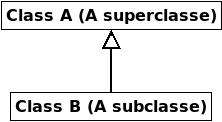
\includegraphics[scale=0.8]{uml1.png} 
\caption{A notação de modelagem UML para a herança} \label{fig:uml1}
\end{center}
\end{figure}

A figura \ref{fig:uml1} ilustra a notação de modelagem UML para a herança, uma linha com uma seta com a ponta oca saindo da subclasse e apontando para a superclasse. A maneira de ler o diagrama é "B herda de A". Em outras palavras, B é uma subclasse direta de A e A é a superclasse direta de B.

A figura \ref{fig:uml2} mostra como você modelaria a hierarquia de herança da classe \emph{Pessoa}. Em geral, chamamos de hierarquia de classes de \emph{Pessoa}, simplesmente. Observe que o nome da classe \emph{Pessoa} está em itálico, isto indica que ela é \textit{abstrata}, enquanto as classes \emph{Professor} e \emph{Estudante} são \textit{concretas}.

\begin{figure}[h]
\begin{center}
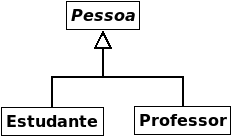
\includegraphics[scale=0.8]{uml2.png} 
\caption{Modelagem do conceito de que \emph{Professor} e \emph{Estudante} herdam de \emph{Pessoa}} \label{fig:uml2}
\end{center}
\end{figure}

\subsection{Dicas e Técnicas para Herança}

As dicas e técnicas a seguir devem lhe ajudar a aplicar hereditariedade de uma forma mais efetiva:

\begin{description}
\item[Procure semelhanças:] Sempre que houver semelhança em duas ou mais classes, seja semelhança nos atributos, seja nos métodos, então, você provavelmente tem uma oportunidade para aplicar a herança.

\item[Procure por classes existentes:] Quando você identifica uma nova classe pode ser que você já tenha uma classe semelhante a ela. Algumas vezes, você pode herdar diretamente de uma classe existente e apenas acrescentar código para as diferenças entre as duas. Por exemplo, suponha que seu sistema de informação universitária também precisa suportar administradores da universidade. A classe \emph{Pessoa} já tem muitas características que uma classe \emph{Administrador} precisa, logo você deve considerar se \emph{Administrador} deve herdar de \emph{Pessoa}.

\item[Siga a regra da sentença:] Uma das frases a seguir deve ter sentido: ``Uma subclasse é um tipo da superclasse'' ou ``Uma subclasse é como uma superclasse''. Por exemplo, faz sentido dizer que um estudante é um tipo de pessoa e um dragão é como um pássaro. Não faz sentido dizer que um estudante é um tipo de veículo, ou é como um veículo, então, a classe \emph{Estudante} provavelmente não deve herdar de \emph{Veiculo}. Se nenhuma das sentenças faz sentido, então você deve ter encontrado um relacionamento de composição ou de associação.

\item[Evite herança de implementação:] Desenvolvedores novatos na orientação a objetos têm uma tendência a errar na aplicação da herança, em geral, num esforço para reusar tanto quanto possível (uma boa motivação). Herança é o conceito mais excitante do repertório de objetos deles, então eles o usam tanto quanto podem. O problema é com o que se chama de herança de implementação ou de conveniência: A aplicação da herança quando a regra da sentença não se aplica e a única justificativa é a de que a subclasse precisa de uma ou mais características da superclasse, a aplicação da herança é mais conveniente do que \textit{refatorar} suas classes. Uma boa regra é reconsiderar a aplicação da regra de herança ``é como'', porque esta é uma justificativa mais fraca.

\item[Herda tudo:] A subclasse deve herdar tudo da superclasse, este conceito é chamado de \emph{herança pura}. Se não, o código torna-se mais difícil de entender e de fazer a manutenção. Por exemplo, digamos que a classe \emph{B} herda de \emph{A}. Para entender \emph{B}, você precisa entender o que é \emph{A} e as características que são acrescentadas em \emph{B}. Se você começar a remover funcionalidade, você precisa entender também o que \emph{B} \textbf{não é}. Isto é muito trabalho e logo a manutenção desse sistema se torna um pesadelo.

\end{description}

\subsection{Herança Simples e Múltipla}

Quando uma classe herda de apenas uma outra classe, dizemos que temos uma \emph{herança simples}. Quando uma classe herda de duas ou mais classes, temos \emph{herança múltipla}. Lembre-se: A subclasse herda todos os atributos e métodos de suas superclasses.

Nem todas as linguagens dão suporte à herança múltipla. C++ é uma das poucas que dá, linguagens como Java, Smalltalk, C\# e Ruby não dão. O ponto é que se sua linguagem de programação não oferece herança múltipla, não use herança múltipla na modelagem. Herança simples resulta em hierarquia de herança que é sempre uma árvore. Herança múltipla resulta em grafos e algumas situações com nomes iguais vindo de superclasses diferentes são muitos complexas. O livro \cite{cpp:ref} comenta sobre algumas das dificuldades enfrentadas para a implementação da herança múltipla no C++.

\begin{figure}[h]
\begin{center}
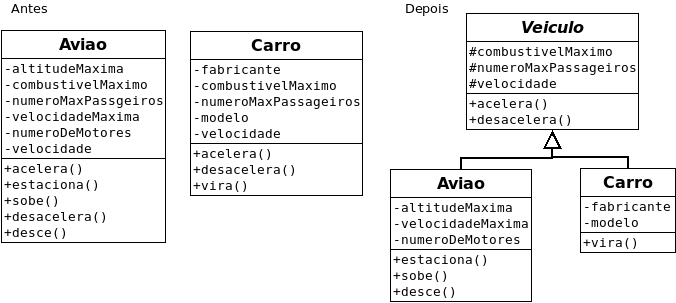
\includegraphics[scale=0.6]{uml3.png} 
\caption{Criação da hierárquia de classes de veículo} \label{fig:uml3}
\end{center}
\end{figure}

Na figura \ref{fig:uml3}, vemos várias semelhanças entre aviões e carros. Ambos têm um número de passageiros, um nível máximo de combustível e ambos podem aumentar ou diminuir a velocidade. Para se aproveitar dessas semelhanças, você pode criar uma nova classe chamada de \emph{Veiculo} e fazer \emph{Aviao} e \emph{Carro} herdar dela. Dizemos que as classes \emph{Veiculo}, \emph{Aviao} e \emph{Carro} formam uma hierarquia de heranças, também chamada de hierarquia de classes. A classe no topo de uma hierarquia de classes (neste caso \emph{Veiculo}) é chamada de raiz ou \emph{classe raiz}. Em Smalltalk e Java, a classe \emph{Object} é a classe raiz de todas as outras classes, direta ou indiretamente.

Observe que existe o método \emph{vira()} em \emph{Carro} e o método \emph{inclina()} em \emph{Aviao}. Virar e inclinar fazem a mesma coisa. Você poderia definir um método \emph{vira()} em \emph{Veiculo} e fazer \emph{Aviao} e \emph{Carro} herdá-lo. Isto implicaria que você teria de requerer que usuários de aviões, isto é, os pilotos, teriam de mudar a terminologia que eles costumam usar. Realisticamente, isto não funcionaria. A melhor solução é manter \emph{vira()} em \emph{Carro} e \emph{inclina()} em \emph{Aviao}.

\begin{figure}
\begin{center}
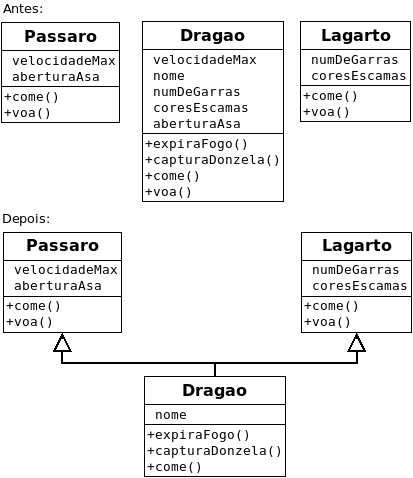
\includegraphics[scale=0.6]{herMultCls.png} 
\caption{Um exemplo de herança múltipla} \label{fig:uml4}
\end{center}
\end{figure}

No Antes: da figura \ref{fig:uml4}, você quer criar uma nova classe \emph{Dragao}. Você já tem as classes \emph{Passaro} e \emph{Lagarto}. Um dragão \textit{é como} um pássaro, pois ambos voam. Um dragão também \textit{é como} um lagarto, ambos têm garras e escamas. Porque dragões têm características de pássaros e lagartos, no Depois: da figura \ref{fig:uml4} temos a classe \emph{Dragao} herdando tanto de \emph{Passaro}, quanto de \emph{Lagarto}. Este é um exemplo de um relacionamento ``é como'' (ou ``parece com''): um dragão é como um pássaro e, também, é como um lagarto.

É importante perceber que a regra de sentença ``é como'' não é perfeita. Por exemplo, faz sentido dizer que uma sequóia é como um arranha-céu já que ambos são altos, têm raízes no chão e balançam ao vento. Entretanto, eles não devem compartilhar uma relação de herança. Também faz sentido dizer que um faixa preta é um artista de artes marciais, mas não faz sentido fazer uma classe \emph{Roupa} herda da classe \emph{Pessoa}.

Observe que o método \emph{come()} foi listado na classe \emph{Dragao}. Embora todos os três tipos de criaturas comam, eles comem cada um de maneira e coisas diferentes. Pássaros comem sementes, lagartos comem insetos e dragões comem cavaleiros em armaduras reluzentes. Porque a maneira de comer dos dragões é diferente da do pássaro e do lagarto, é necessário \textit{redefinir} (sobrescrever) a definição do método \emph{come()}. A ideia geral é que uma subclasse precisa sobrescrever um atributo ou um método sempre que ela usa aquele dado ou executa aquele método de uma maneira diferente da sua superclasse\footnote{A programação de jogos é um dos poucos domínios em que herança múltipla faz muito sentido.}.

\subsection{Classes Abstratas e Concretas}

Na figura \ref{fig:uml3}, a classe \emph{Veiculo} está marcada como abstrata (o nome está em itálico, em versões mais antigas de UML, você poderia usar a restrição \emph{\{abstract\}}), enquanto \emph{Aviao} e \emph{Carro} não são. Dizemos que 
\emph{Veiculo} é uma classe abstrata, enquanto \emph{Aviao} e \emph{Carro} são classes concretas. A diferença principal entre classes abstratas e concretas é que objetos podem ser instanciados (criados) de classes concretas, mas não de classes abstratas. Por exemplo, no domínio do seu problema, você tem aviões e carros, mas não tem nada que é apenas um veículo (se algo não é um avião ou um carro, você não se interessa por ele). Isto significa que seu software instanciará objetos aviões e carros, mas não objetos veículos. Classes abstratas são modeladas quando você precisa criar uma classe que implementa características comuns a duas ou mais classes. Observe que ao usar padrões de projeto, muitos deles definem interfaces que são classes abstratas. No modelamento é normal projetar classes pelas suas responsabilidades e essas classes não serem instanciáveis até que se defina uma forma de implementação concreta para estas responsabilidades.

Não é necessário se preocupar com se uma classe é abstrata quando estamos modelando, assumimos que faremos a coisa certa quando vier a hora de implementar a classe, o que numa equipe de projeto ágil pode ser minutos depois de modelá-la. Usar itálico para indicar que uma classe é abstrata é uma escolha infeliz do pessoal da OMG. Como \cite{uml:destilado} disse, quando você está modelando num quadro negro ou num papel (lembre-se que a prática de modelagem ágil diz: \textit{use a ferramenta mais simples}), você precisa usar a notação antiga, \emph{\{abstract\}}, ou \emph{<<abstract>>}. Se você realmente pretende que uma classe seja abstrata, a maioria das linguagens OO permite que se declare que uma classe é abstrata e ela nunca poderá ser instanciada.

Enquanto \cite{Ambler:TOP:3ed} não se preocupa com o fato da classe ser abstrata na modelagem, \cite{DP:explained} dá uma forte enfase no uso de classes abstratas para representa a ideia de comunalidade e a definição da interface de programação (API - Application Programming Interface) entre os componentes de software. Na prática, devemos observar as classes e na medida que o desenvolvimento for avançando, com o surgimento da necessidade de mais classes, devemos considerar se classes diferentes apresentam responsabilidades semelhantes e se não faz sentido unificá-las em uma mesma classe abstrata. Devemos, entretanto, evitar os excessos que levam à herança de implementação. O uso de padrões de projeto pode auxiliar a determinar quais são as classes abstratas interessantes na solução de um problema. As alterações necessárias para usar a comunalidade de diversas classes e forma uma interface unificada por uma classe abstrata é uma forma de refatoramento que permite reduzir, em geral, acoplamentos.

\section{Persistência}

Persistência foca na questão de como fazer com que os objetos estejam disponíveis para uso futuro pelo software. Em outras palavras, como salvar objetos na memória permanente. Para fazer um objeto ser permanente, você deve salvar os valores de seus atributos na memória permanente (tais como num banco de dados ou num arquivo) e também qualquer informação necessária para manter seus relacionamentos (agregação, herança e associação) nos quais está envolvido. Em outras palavras, você precisa salvar as propriedades apropriadas na memória permanente. Além de salvar objetos, persistência também se preocupa em recuperá-los e apagá-los.

Do ponto de vista de desenvolvimento, existem dois tipos de objetos: \textbf{objetos persistentes} que continuam por aí e \textbf{objetos transitórios} que se vão. Por exemplo, um \emph{Cliente} é uma classe persistente. Você quer salvar objetos clientes em algum tipo de memória permanente de modo que você possa trabalhar com eles de novo no futuro. Uma tela de edição de um cliente, entretanto, é um objeto transitório. Sua aplicação cria uma tela de edição de cliente, mostra-a e livra-se dela depois que o usuário terminou de editar os dados do cliente.

As seguintes dicas e técnicas devem ajudar a entender e aplicar o conceito de persistência melhor:

\begin{enumerate}
\item \textbf{Classes do negócio/ do domínio do problema são geralmente persistentes.} Você  naturalmente precisa manter um registro permanente (ou persistente) de instâncias de classes do mundo real como \emph{Estudante}, \emph{Professor} e \emph{Disciplina}.

\item \textbf{Classes da interface usuário são geralmente transitórias.} Classes da interface de usuário (telas e relatórios) são, em geral, transitórios. Telas são criadas e exibidas quando necessário e, então, quando não estão mais em uso, elas são destruídas (removidas da memória). Objetos relatórios são criados, eles adquirem os dados de que precisam, manipulam os dados e imprimem os dados. Depois disto, o objeto relatório é destruído. Note que, às vezes, você pode precisar manter um registro (\textit{log}) da impressão do relatório e de quem mandou fazer a impressão, o registro (\textit{log}) neste caso deve ser permanente.

\item \textbf{Você precisa armazenar tanto os atributos quanto as associações.}
Quando um objeto é escrito no disco, você obviamente precisa armazenar os valores dos seus atributos. Entretanto, você também deve armazenar informações sobre seus relacionamentos/associações com os quais o objeto está envolvido. Por exemplo, Bia está cursando Bio-medicina e Enfermagem, então você precisa se assegurar que quando você for armazenar o objeto Bia no disco, o software vai registrar que ela está matriculada nestas duas disciplinas.
\end{enumerate}

\section{Relacionamentos}

\begin{figure}[ht]
\begin{center}
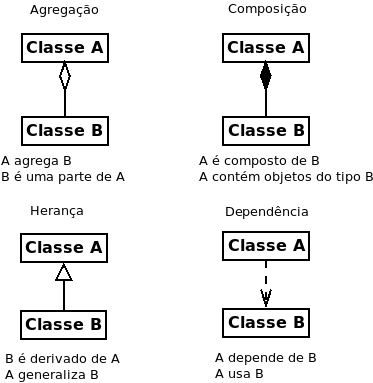
\includegraphics[scale=0.65]{clsRelac.png}
\end{center}
\caption{Resumo dos diagramas de relacionamento.} \label{fig:relac}
\legend{Fonte: \cite{uml:j2ee}}
\end{figure}

No mundo real, os objetos têm relacionamentos uns com os outros. Os relacionamentos entre os objetos são importantes porque nos ajudam a definir como os objetos interagem uns com os outros. Por exemplo, estudantes \textit{se matriculam} em disciplinas, professores \textit{ensinam} disciplinas, criminosos \textit{roubam} bancos, políticos \textit{beijam} bebes e capitães \textit{comandam} espaçonaves. \textit{Se matriculam}, \textit{ensinam}, \textit{roubam}, \textit{beijam} e \textit{comandam} são todos verbos que definem associações entre objetos. Você quer identificar e potencialmente documentar estes relacionamentos; assim, você pode ganhar um melhor entendimento de como os objetos interagem uns com os outros. A figura \ref{fig:relac} resume as notações para relacionamentos entre duas classes.

Você não precisa apenas identificar os relacionamentos entre as classes, você deve também descrever o relacionamento. Por exemplo, não é suficiente saber que os estudantes se matriculam em disciplinas. Quantas disciplinas os estudantes podem cursar? Nenhuma, uma ou várias? Além disso, relacionamentos são vias com circulação nos dois sentidos: Não apenas os estudantes se matriculam em disciplinas, mas também disciplinas têm estudantes matriculados. Isto leva a questões como quantos estudantes podem ser matriculados numa dada disciplina e é possível ter uma disciplina sem nenhum estudante? Isto implica em que você deve também identificar a cardinalidade e a opcionalidade de um relacionamento. Cardinalidade representa o conceito ``quantos'', opcionalidade representa o conceito ``se você deve ter algo''. É importante observar que a UML escolheu combinar os conceitos de opcionalidade e cardinalidade num único conceito de \emph{multiplicidade}.

\noindent \framebox{
\begin{minipage}{16cm}

\textbf{Considere Opcionalidade e Cardinalidade Separadamente}

A experiência mostra que é melhor considerar separadamente estes dois conceitos: Para cada direção de uma associação é importante se a associação deve existir (opcionalidade) e quantos podem possivelmente existir (cardinalidade)? Por exemplo, considere a associação ``ensina'' entre professores e disciplinas, devemos perguntar:
\begin{itemize}
\item Um professor deve ensinar uma disciplina, ou pode haver professor que não ensina nenhuma disciplina?
\item Quantas disciplinas um professor pode ensinar no máximo?
\item Toda disciplina deve ser ensinada por um professor, ou é possível que alguém que não é professor a ensine?
\item Mais de um professor pode ensinar numa disciplina? Quantos?
\item Existem disciplinas que exigem que mais de um professor as ensinem?
\end{itemize}
\end{minipage}
}

\subsection{Associações}

\begin{figure}
\begin{center}
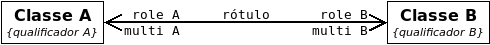
\includegraphics[scale=0.6]{assocCls.png} 
\caption{Notação simplificada da modelagem de associações em diagramas de classes em UML} \label{fig:uml5}
\end{center}
\end{figure}

Uma associação é um relacionamento persistente entre duas ou mais classes ou objetos. Quando você modela associações em diagramas de classes de UML, você as mostra como uma linha fina conectando duas classes, como você pode ver na figura \ref{fig:uml5}. Associações podem facilmente ficar bastante complexas; Consequentemente, você pode exibir várias coisas a respeito deles nos seus diagramas. A figura \ref{fig:uml6} mostra os itens comuns a modelar numa associação:

\begin{figure}
\begin{center}
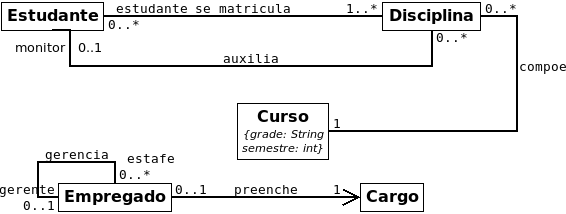
\includegraphics[scale=0.6]{assocCls2.png} 
\caption{Diversos exemplos de associação} \label{fig:uml6}
\end{center}
\end{figure}

\begin{description}
\item[Direcionalidade:] Setas com ponta vazada indicam a direcionalidade da associação. Quando existe uma seta, a associação é unidirecional: Ela só pode ser percorrida numa direção (na direção da seta). Quando não tem seta ou tem dupla seta, a associação é bidirecional: Ela pode ser percorrida em ambos sentidos. Embora você deva indicar com as duas setas, é prática comum deixar de colocar as setas nas associações bi-direcionais. Exemplos das duas notações para associações bidirecionais estão na figura \ref{fig:uml6}. Neste texto, adotaremos a prática da modelagem ágil -- exiba os modelos de maneira simples -- nas associações bidirecionais usaremos linhas sem setas. Recomenda-se a escolha de uma convenção e mantê-la.

\item[Rótulo:] O rótulo que é opcional, é tipicamente composto por uma ou duas palavras descrevendo a associação. A leitura do nome de uma classe, do rótulo e do nome da outra classe deve produzir uma frase que descreva o relacionamento, por exemplo, \emph{Professor ensina Disciplina}. Evite rótulos genéricos como \textit{tem} ou \textit{comunica com}, tanto quanto possível.

\item[Multiplicidade:] A multiplicidade da associação é rotulada em ambas pontas da linha, uma multiplicidade para cada direção. A tabela \ref{tab:uml:mult} mostra os principais indicadores de multiplicidade que podem ser usados.

\item[Papel:] O papel (\textit{role}), o contexto que cada objeto assume na associação, pode ser indicado na ponta da associação.

\item[Qualificador:] Um qualificador é um valor que seleciona um objeto do conjunto de objetos relacionados através de uma associação. Por exemplo, na figura \ref{fig:uml6}, a associação \emph{compõe} de \emph{Disciplina} para \emph{Curso} é qualificada pela combinação dos atributos \emph{grade} e \emph{semestre} (potencialmente implementada pela \emph{Disciplina}). Qualificadores são opcionais e na prática raramente modelados\footnote{Tanto que a ferramenta Dia usada para criar os nossos diagramas não possui a opção de incluí-los, a notação usada no diagrama foi a de uma \textit{restrição}.}.

\end{description}

\begin{table}
\caption{Indicadores de Multiplicidade do UML} \label{tab:uml:mult}
\begin{center}
\begin{tabular}{l l}

\textbf{Indicador} & \textbf{Significado} \\
\hline

0..1 & Zero ou um \\
1 & Apenas um \\
0..* & Zero ou mais \\
1..* & Um ou mais \\
n & Apenas n (onde $n>1$) \\
0..n & Zero a n (onde $n>1$) \\
1..n & Um a n (onde $n>1$)\\
\hline

\end{tabular}
\end{center}
%\legend{Fonte: \citeonline{Ambler:TOP:3ed}}
\end{table}

Observe o diagrama de classes da figura \ref{fig:uml6}, que mostra diversas classes e as associações entre elas. Eis como você leria as associações:
\begin{itemize}
\item Um estudante se matricula em uma ou mais disciplinas;
\item Uma disciplina tem 0 ou mais estudantes matriculados;
\item Um estudante, como monitor, pode auxiliar em zero ou mais disciplinas;
\item Uma disciplina pode ter 0 ou um estudante que age como monitor;
\item Uma disciplina compõe um curso;
\item Um curso é composto por zero ou mais disciplinas;
\item Um empregado possui um cargo;
\item Um cargo pode ser preenchido por um empregado (alguns cargos podem não está preenchidos);
\item Um empregado pode ser gerenciado por um um outro empregado, o gerente (o presidente da companhia é o único sem um gerente); e
\item Um empregado gerencia zero ou mais empregados.
\end{itemize}

Diversos pontos importantes estão mostradas na figura \ref{fig:uml6}. Primeiro, observe que é possível ter mais de uma associação entre duas classes: As classes \emph{Estudante} e \emph{Disciplina} têm as associações \emph{se\_matricula} e \emph{auxilia} entre elas. Você se interessa nestes dois relacionamentos entre estas classes para o seu sistema de informação da universidade, logo, você precisa modelar ambas as associações.

Segundo, é válido que a mesma classe se envolva nas duas pontas de uma associação; Isto é chamado de associação recursiva ou auto-associação (\citeonline{uml:destilado}). Um exemplo perfeito disto é a associação \emph{gerencia} que a classe \emph{Empregado} tem consigo mesma. A maneira de ler isto é a de que um empregado qualquer pode gerenciar outros e ele, ou ela, pode ser gerenciado(a) por outro empregado.

Terceiro, algumas vezes, o sentido de uma associação é único, como pode ser visto na figura \ref{fig:uml6} pela associação \emph{preenche} entre \emph{Empregado} e \emph{Cargo}. A implicação é que o objeto empregado sabe o cargo que preenche, mas o objeto cargo não precisa saber qual empregado o está preenchendo. Esta é uma associação dita unidirecional, uma associação que só é percorrida numa única direção. Se você não tiver um requisito para que se percorra uma associação nos dois sentidos, por exemplo, cargos não precisam colaborar com objetos empregados, então use uma associação unidirecional. Veremos que associações unidirecionais requerem menos trabalho para serem implementadas.

\subsection{Modelagem do Desconhecido}

Não importa o quanto é bom o trabalho que você realiza, pode-se com quase certeza absoluta garantir que você perdeu algum detalhe dos relacionamentos dos seus objetos. Então, o que pode ser feito é: \textit{Faça e torça para que dê certo?} Óbvio que não. Você vai voltar aos seus usuários e perguntar para eles como estão as coisas, não? O problema é lembrar de voltar aos seus usuários. A solução: Marcar como \emph{desconhecido agora} colocando um ponto de interrogação na parte do relacionamento em que você tem uma dúvida. Por exemplo, na figura \ref{fig:uml7}, você acredita que zero ou mais empregados podem preencher um cargo. Você sabe que um cargo pode não está preenchido, mas não tem certeza se um cargo pode ser preenchido por uma ou mais pessoas. Existe compartilhamento de emprego na organização? Existem cargos genéricos como Faxineiro, que é preenchido por várias pessoas? Ou é realmente, uma pessoa por cargo, como estamos mostrando atualmente? Porque você não sabe com certeza ainda, você marca o relacionamento com um ponto de interrogação, indicando que você deve retorna para ele mais tarde e checar seu \emph{chute educado}. Observe que UML não inclui pontos de interrogação como parte da notação, é apenas uma técnica que Ambler descobriu ser muito útil na prática -- idealmente, você não deve adivinhar ou supor coisas sem falar antes com quem está adquirindo o sistema (o \textit{stockholder}), mas se você precisar, então marque sua suposição no seu trabalho e procure resolver a dúvida o quanto antes.

\begin{figure}[h]
\begin{center}
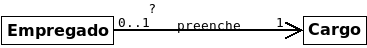
\includegraphics[scale=0.6]{assocCls3.png} 
\caption{Indicação de desconhecido} \label{fig:uml7}
\end{center}
\end{figure}

\subsection{Como Associações São Implementadas}

Associações são mantidas pela combinação de atributos e métodos. Os atributos armazenam as informações necessárias para manter o relacionamento e os métodos atualizam os atributos. Por exemplo, a classe \emph{Estudante} da figura \ref{fig:uml6} potencialmente tem um atributo \emph{matriculado\_em}, talvez, um \textit{array}, que é usado para guardar em quais objetos \emph{Disciplina} o estudante está matriculado. A classe \emph{Estudante} pode também ter métodos como \emph{adicionaDisciplina()} e \emph{removeDisciplina()} para adicionar ou remover objetos disciplinas do \textit{array}. A classe Disciplina teria um atributo similar \emph{estudantes} e métodos \emph{adicionaEstudante()} e \emph{removeEstudante()} para manter a associação no sentido oposto. Tudo isto tem uma implicação importante: assim como atributos e métodos são herdados, associações também são.

Na figura \ref{fig:uml6}, a associação unidirecional \emph{preenche} entre \emph{Empregado} e \emph{Cargo} é mais fácil de implementar porque você só precisa percorrer num único sentido: Do \emph{Empregado} para o \emph{Cargo}. Logo, \emph{Empregado} tem um atributo \emph{cargo} e métodos \emph{setCargo()} e \emph{getCargo()} para implementar a associação. Nada precisa ser acrescentado à classe \emph{Cargo}, porque não existe a necessidade de objetos cargos colaborarem com objetos empregados. Logo, não há a necessidade de acrescentar código para implementar a associação no outro sentido.

\noindent \framebox{
\begin{minipage}{16cm}
\textbf{Não mostre atributos e métodos para implementar associações}

É um estilo comum supor que existem atributos e métodos para implementar associações, você não precisa mostrá-los nos seus diagramas. Considere estabelecer convenções para os nomes destes atributos e métodos. Tipicamente, o nome do papel, ou o nome da classe, para o nome do atributo e nomes de métodos como \emph{adicionaNomeAtributo()} e \emph{removeNomeAtributo()} para associações múltiplas e \emph{setNomeAtributo()} e \emph{getNomeAtributo()} para associações simples.
\end{minipage}
}

\subsection{Propriedades}

Em UML 2, uma propriedade é um valor nomeado que denota uma característica de um elemento (tal como uma classe ou um componente). Atributos e associações, inclusive composição, são propriedades. Por exemplo, o nome de um estudante é uma propriedade importante da classe \emph{Estudante}. O fato de estudantes se matricularem em disciplinas também é uma propriedade importante da classe \emph{Estudante}. Logo, faz sentido atributos e relacionamentos serem propriedades de classes. Lembre-se, também, que a implementação de associações se faz, em parte, através de atributos.

\subsection{Agregação e Composição}

Algumas vezes, um objeto é feito de outros. Por exemplo, um avião é feito de fuselagem, asas, motores, trem de pouso, \textit{flaps}, ... Uma entrega contém um ou mais pacotes. Uma equipe de projeto constitui-se de dois ou mais empregados. Estes são exemplos de agregação, que é representada pelo relacionamento \emph{é parte de}. Um motor é parte de um avião, um pacote é parte de uma entrega e um empregado é parte de uma equipe.

Composição é um tipo forte de agregação no qual o ``todo'' é completamente responsável pelas partes e cada objeto ``parte'' só é associado a um objeto ``todo''. Por exemplo, em qualquer instante, um motor só está associado a um único avião. Além disso, nenhum outro objeto iria colaborar com o objeto motor, além do seu objeto avião. Por exemplo, objetos passageiros do avião não podem pedir para aumentar diretamente a velocidade de um motor.

\begin{figure}[h]
\begin{center}
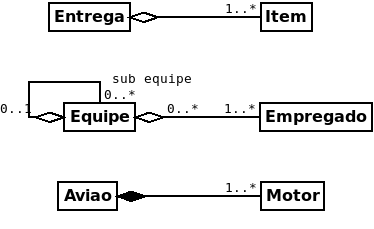
\includegraphics[scale=0.6]{agreg.png} 
\caption{Exemplos de agregação} \label{fig:uml8}
\end{center}\end{figure}

Em UML 1, você podia modelar agregação e composição, mas no UML 2, a notação da agregação caiu. Embora isto pareça uma boa ideia, porque muita gente confundia os dois conceitos, suspeita-se que agregação continue a ser usada em diagramas de classe de UML por mais um tempo, a agregação é popularmente modelada desde 1997, quando a UML se popularizou. A figura \ref{fig:uml8} mostra exemplos de ambos -- a agregação era exibida como uma seta com uma ponta em losângulo vazio e composição com um losângulo cheio. O losângulo está conectado à classe toda. Agregação é simplesmente um tipo de associação. Você ainda tem de modelar as multiplicidades e os papéis. Deixar de indicar a multiplicidade de uma associação é permitido, mas não é recomendável. Por exemplo, na figura \ref{fig:uml8}, a multiplicidade não é indicada nem para entregas, nem para aviões, nestes casos, a multiplicidade implícita é 1.

Assim como associações são vias de duplo sentido, também as agregações são. Além disso, as associações de agregação/composição mostradas na figura \ref{fig:uml8} são lidas de maneira similar:
\begin{itemize}
\item Um item é parte de uma e apenas uma entrega;
\item Uma entrega é composta por um ou mais itens;
\item Um motor é parte de um e apenas um avião;
\item Um avião tem um ou mais motores;
\item Um empregado pode ser parte de uma ou mais equipes;
\item Uma equipe é constituída de um ou mais empregados;
\item Qualquer equipe pode fazer parte de uma equipe maior; e
\item Uma equipe pode ser constituída de subequipes menores.
\end{itemize}

É importante conhecer a antiga notação para agregação. Mesmo que não a usemos mais.

As dicas a seguir ajudam a modelar adequadamente a composição:
\begin{enumerate}
\item \textbf{Aplique a regra da sentença:} O primeiro teste é que a frase ``a parte \emph{é parte do} todo'' deve fazer sentido. Por exemplo, faz sentido dizer: Um motor \emph{é parte de} um avião. Entretanto, não faz sentido dizer que um empregado \emph{é parte de} um cargo, ou um cargo \emph{é parte de} um empregado, por isso que é mais apropriado usar uma associação como na figura \ref{fig:uml6}. Se a frase não faz sentido, a composição não é apropriada. Herança ou associação devem ser usadas nesse caso.

\item \textbf{O todo deve gerenciar as partes:} O segundo teste, supondo que o primeiro tenha sido aprovado, é se o todo gerencia as partes. Por exemplo, um avião deve gerenciar os motores; você não deseja que um passageiro no avião seja capaz de manipular os motores.

\item \textbf{Você deve se interessar pela parte:} Um objeto pode fazer parte no mundo físico, mas você pode não estar interessado nele, logo, não o modele. Por exemplo, um sistema de manutenção de aeronaves pode ser interessante para os registros de cada motor, guardando as informações de manutenção dos motores. Por outro lado, o sistema de controle de tráfego aéreo não tem informações interessantes para os motores. Logo, um motor não vai aparecer no diagrama de classes do sistema de controle de tráfego aéreo.

\item \textbf{Mostre a multiplicidade e os papéis:} Assim como você mostra a multiplicidade e os papéis numa associação, você deve mostrá-los numa composição.

\item \textbf{Composição é herdada:} Associações de composição, assim como, associações comuns, são implementadas por atributos e métodos, portanto, podem ser herdadas.
\end{enumerate}

\subsection{Dependências}

Existem dois tipos de relacionamentos: persistente e transitório. A diferença principal é a de que associações persistentes devem ser salvas, enquanto relacionamentos transitórios têm natureza temporária e não precisam ser salvos.

Relacionamentos persistentes são permanentes, ou, pelo menos, semi-permanentes, por natureza. Um relacionamento de objetos é persistente se a informação para mantê-lo é salva em memória permanente. Por exemplo, o relacionamento \emph{se\_matricula} entre estudantes e disciplinas é persistente. Isto é uma informação de negócio importante que deve ser armazenada no disco. O relacionamento \emph{ensina} entre professores e disciplinas é persistente pelo mesmo motivo. Todos os relacionamentos que vimos até agora são persistentes.

Associações transitórias são temporárias por natureza. Elas não são salvas no armazenamento permanente. Relacionamentos transitórios envolvem, geralmente, mas não sempre, pelo menos um objeto transitório, tal como uma tela, ou um relatório. A razão para isto é simples: Se você não precisa persistir um objeto, então, você não precisa persistir seus relacionamentos.

Relacionamentos transitórios existem entre objetos por uma razão apenas: Os objetos precisam colaborar entre eles. Para um objeto colaborar com outro objeto, ele precisa conhecê-lo. Isto significa que deve existir, ou um relacionamento entre os objetos, ou um relacionamento do tipo ``parte-de'' entre os dois objetos. Quando não há uma associação persistente  entre dois objetos, mas eles colaboram um com o outro, você modela uma relação de dependência entre as duas classes.

\begin{figure}[h]
\begin{center}
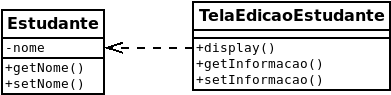
\includegraphics[scale=0.7]{classDep.png}
\end{center}
\caption{Dependência entre duas classes.} \label{fig:clsDep}
\end{figure}

A figura \ref{fig:clsDep} mostra um relacionamento de dependência -- modelada pela linha tracejada com uma seta aberta -- entre as classes \emph{Estudante} e \emph{TelaEdicaoEstudante}, representando o relacionamento transitório entre um objeto tela de edição de estudante usado para atualizar o objeto estudante. A tela de edição obtém a informação atual do objeto estudante, mostra no modo de edição e atualiza a informação nova quando termina a edição. O relacionamento transitório entre o objeto tela de edição e o objeto estudante existe enquanto a informação do estudante é exibida na tela. Quando a tela é fechada, o relacionamento deixa de existir (a tela também não existe mais) e os objetos transitórios provavelmente já foram destruídos.

Associações transitórias podem também ocorrer entre objetos persistentes. Por exemplo, na figura \ref{fig:seq}, uma associação transitória implícita
existe entre o objeto estudante e o objeto curso (o estudante é passado como um parâmetro para o curso, para saber se ele atende as condições de pré-requisitos). Esta associação não foi ilustrada na figura \ref{fig:uml6} porque o conceito não foi introduzido naquele momento. Por consistência, as associações transitórias também  precisam ser modeladas.

\begin{figure}
\begin{center}
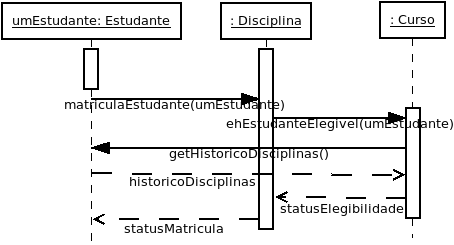
\includegraphics[scale=0.65]{clsSeq.png}
\end{center}
\caption{Diagrama de sequência mostrando mensagens entre objetos.} \label{fig:seq}
\end{figure}

\section{Colaboração}

Classes precisam, em geral, trabalhar juntas para cumprirem suas responsabilidades. Na verdade, são os objetos, as instâncias das classes que trabalham juntas. Colaboração entre objetos ocorre quando um objeto pede ao outro informações ou para o outro realizar algo. Por exemplo, um avião colabora com seus motores para poder voar. Para o avião ir mais rápido, ele pede para os motores girarem mais rápido. Quando um avião precisa desacelerar, os motores precisam desacelerar. Se o avião não colaborasse com seus motores, ele não voaria.

Objetos colaboram uns com os outros pelo envio de mensagens. Uma mensagem é tanto um pedido para fazer alguma coisa, quanto um um pedido por informações. Mensagens são modeladas por diagramas de sequência e diagramas de comunicação (diagramas de colaboração em UML 1.x) em UML. A figura \ref{fig:seq} mostra um diagrama de sequência simples. Nele, você vê como um estudante requer a matrícula numa disciplina: O objeto disciplina de sua parte manda uma mensagem para o objeto curso com o qual está associado para saber se o estudante pode se matricular na disciplina (checar pré-requisitos, por exemplo). A figura \ref{fig:comm} mostra o mesmo exemplo, mas na forma de diagrama de comunicação.

\begin{figure}[h]
\begin{center}
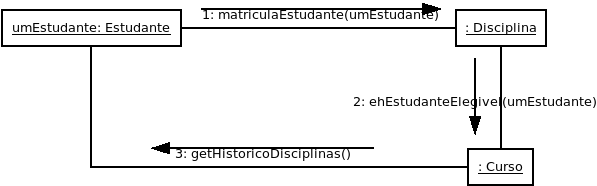
\includegraphics[scale=0.6]{clsComm.png}
\end{center}
\caption{Diagrama de comunicação exibindo as mensagens.} \label{fig:comm}
\end{figure}

Vejamos alguns detalhes sobre o diagrama de sequência, as caixas no topo do diagrama representam classificadores, no caso, mais precisamente, objetos. As linhas tracejadas penduradas nas caixas são chamadas de \textit{linha de vida} dos objetos e representam o intervalo de tempo de vida do objeto no cenário modelado. Objetos são rotulados no formato \emph{nome: classe} onde o \emph{nome} é opcional (objetos que não receberam nomes no diagrama são chamados de \textit{objetos anônimos}). A instância de \emph{Estudante} recebeu um nome porque ela é usada como parâmetro numa mensagem, já as instâncias de \emph{Disciplina} e \emph{Curso} não precisam ser referenciadas em nenhuma parte do diagrama e, portanto, podem ser anônimas. As  mensagens são indicadas por setas rotuladas, o rótulo é a assinatura do método. Valores de retorno são indicados opcionalmente por seta com linha tracejada e um rótulo indicando o valor de retorno. Valores de retorno estão representados na figura \ref{fig:seq}, mas não na \ref{fig:seq2}. Em metodologias ágeis, devemos manter os diagramas simples e assumir que o valor de retorno volta. O sequenciamento das mensagens é dado pela ordem das próprias mensagens, começando no topo a esquerda do diagrama.

Diagramas de comunicação têm uma notação similar aos diagramas de sequência. Objetos são indicados da mesma maneira, embora eles sejam conectados por linhas de associação sem rótulos. As mensagens são indicadas com setas de novo, embora não conectem os objetos (não há linhas de vida nos diagramas de comunicação/colaboração). A sequência de mensagens é opcionalmente indicada colocando um número na frente do nome da mensagem. Na figura \ref{fig:comm}, vemos a mesma sequência de mensagens que a da figura \ref{fig:seq}.

As dicas e técnicas a seguir devem ajudar a modelar de maneira efetiva as colaborações:

\begin{enumerate}
\item \textbf{Deve ter algum tipo de relacionamento.} A única maneira de um objeto poder mandar um mensagem para um outro é se o conhece antes. No mundo real, você não pode pedir ajuda a alguém se você não sabe como contactá-lo. O mesmo princípio se aplica a objetos. Deve existir um associação, talvez uma agregação, entre as duas classes para que as instâncias (objetos) sejam capazes de colaborar.

\item \textbf{Deve ter um método correspondente no objeto alvo.} Colaborações são implementadas através de chamadas de métodos, isto implica que o método deve existir no objeto alvo para ele ser chamado. Para um objeto poder receber um pedido de informação, ele deve ter um método que retorna esta informação. Por exemplo, na figura \ref{fig:seq}, a mensagem \emph{ehEstudanteElegivel()} é enviada para o objeto curso, logo na classe \emph{Curso} deve haver uma implementação do método \emph{ehEstudanteElegivel()}. Se desejamos que um objeto faça algo, ele deve ter um método que o faça. De modo similar, na figura \ref{fig:seq}, observe que a mensagem \emph{matriculaEstudante()} é enviada a objetos disciplinas, logo a classe \emph{Disciplina} deve ter um método \emph{matriculaEstudante()}.

\item \textbf{Pode haver um valor de retorno.} Se a colaboração é um pedido de informação, então deve haver o retorno de um valor (a informação pedida). Este fato deve ser incluída na documentação do método e, opcionalmente, será indicada no diagrama de sequência como uma linha tracejada. Valores de retorno não são modelados em diagramas de colaboração porque eles tendem a poluir os diagramas.

\item \textbf{Pode ter ou não parâmetros.} Algumas mensagens têm parâmetros, outras não. Lembre-se de que mensagens são efetivamente uma chamada de método (função). Assim como funções têm parâmetros, métodos também têm. Por exemplo, na figura \ref{fig:seq}, um objeto estudante passa a si mesmo como um parâmetro quando chama a mensagem \emph{matriculaEstudante()} do objeto \emph{Disciplina}. Na figura \ref{fig:seq2}, o objeto entrega não precisa passar qualquer parâmetro quando pede ao objeto item o seu preço.

\begin{figure}[h]
\begin{center}
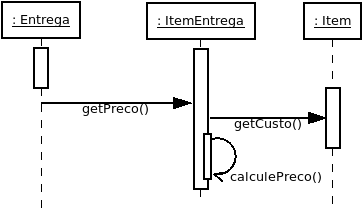
\includegraphics[scale=0.65]{seq2.png}
\end{center}
\caption{Diagrama de sequência.} \label{fig:seq2}
\end{figure}

\item \textbf{Mensagens mostram a colaboração, não o fluxo de dados.} Mensagens são pedidos. Elas não são fluxos de dados. Diagramas de processo (diagramas de fluxo de dados) do mundo estruturado mostram fluxos de dados, que são movimentos de dados de uma parte do sistema para outra.

\item \textbf{Algumas vezes o alvo precisa colaborar.} O receptor de uma mensagem pode não ser capaz de atender a um pedido completamente  e pode precisar colaborar com outros objetos para cumprir sua responsabilidade. Por exemplo, na figura \ref{fig:seq}, o objeto disciplina precisou interagir com o objeto curso do qual ela faz parte para matricular um estudante. Isto é perfeitamente válido.

\item \textbf{Cada método deve fazer alguma coisa.} É importante que cada objeto colaborador deve sempre fazer algo, não apenas encaminhar a mensagem para outro objeto, algo chamado de uma passarela (\textit{passthrough}). Passarelas resultam em \textit{código espaguete} que pode ser difícil para dar manutenção. Algumas vezes, \textit{delegação}, um padrão de projeto, faz sentido, mas, enquanto você for um principiante, é melhor evitar.

\item \textbf{Um objeto pode colaborar consigo mesmo.} Objetos frequentemente se enviam mensagens para obter informações e/ou para fazer alguma coisa. Isto é como uma função chamando uma outra em uma linguagem procedural como o C. Na figura \ref{fig:seq2}, o objeto \emph{ItemEntrega} se manda uma mensagem para calcular o preço (provavelmente, o preço do item vezes o número de itens a ser entregue).

\end{enumerate}

\section{Acoplamento}

Acoplamento é uma medida do quanto dois itens, tais como classes ou métodos, estão relacionados entre eles. Quando uma classe depende de uma outra, dizemos que elas estão acopladas. Quando uma classe interage com uma outra, mas não conhece nada sobre os detalhes de implementação da outra, dizemos que elas são fracamente acopladas. Quando uma classe se baseia na implementação (isto é, tem acesso direto aos atributos da outra), dizemos que elas estão fortemente acopladas.

Na discussão de como \emph{Estudante} pode implementar o método \emph{se\_matricula()}: Ele pode acessar diretamente o atributo \emph{listaDeEstudantes} de \emph{Disciplina}, ou pode enviar uma mensagem para objetos \emph{Disciplina} pedindo para matricular o estudante na disciplina. Acessando diretamente e mudando o atributo \emph{listaDeEstudantes} pode economizar alguns ciclos de CPU e rodar mais rápido, mas assim que a implementação daquele atributo mudar (passando de um \textit{array} para uma \textit{lista encadeada}, por exemplo), seu código da classe \emph{Estudante} também vai ter de mudar. Isto não é muito bom. O problema básico é que quando duas classes são fortemente acopladas, uma mudança numa, requer uma mudança na outra. Isto, por sua vez, pode requerer uma mudança em outra classe, e em outra, ... Acoplamento forte é uma das causas para a manutenção de código ser complexa. O que deveria ser uma troca simples de manutenção pode levar meses para estabilizar, se é que vai ficar estável. É incrível a quantidade de código que existe que ninguém quer tocar com medo de quebrá-lo. Por exemplo, lembre-se do ano 2000 (bug do milênio, que não era no milênio).

Frequentemente, os desenvolvedores são seduzidos pelo lado negro da força e decidem escrever código fortemente acoplado. Isto só se justifica quando você está desesperado em reduzir todos códigos redundantes do seu programa. Por exemplo, \textit{drivers} de bancos de dados são fortemente acoplados aos sistemas de arquivos do sistema operacional onde o banco de dados está instalado. Se você puder salvar uns microssegundos no acesso aos dados, isto pode ser significativo ao acessar centenas de milhares de objetos.

\section{Coesão}

Coesão é uma medida do quanto um item, tal como uma classe ou um método, faz sentido. Uma boa medida da coesão de algo é quanto tempo leva para descrevê-lo numa frase: quanto mais tempo levar, menos coeso ele é. Você deseja projetar classes e métodos com alto grau de coesão. Em outras palavras, você deseja classes e métodos cuja descrição seja bem clara.

Um método é bastante coeso se ele faz uma coisa e apenas esta coisa. Por exemplo, na classe \emph{Estudante}, você teria métodos para matricular estudantes em disciplinas e remover estudantes de disciplinas. Cada um desses métodos faze uma coisa e apenas esta coisa. Você poderia escrever um método que faz as duas coisas e chamá-lo, por exemplo, de \emph{mudaStatusDisciplina()}. O problema com esta solução é que o código ia ficar mais complexo do que com os dois métodos separados. Isto significa que seu código ia ficar mais difícil de ser entendido e, portanto, de fazer a manutenção ia ficar mais complicada. Lembre-se de que você deve simplificar a manutenção, não torná-la mais complexa.

\noindent \framebox{ \begin{minipage}{16cm}
\textbf{Nomes de métodos indicam o grau de coesão}

O nome de um método, em geral, indica o quanto ele é coeso. Sempre que você encontrar uma combinação forte verbo/complemento para ser usada como nome de método, há grandes chances do método ser fortemente coeso. Por exemplo, leve em consideração métodos como \emph{getNome()}, \emph{printNome()}, \emph{matriculaDisciplina()} e \emph{desisteDisciplina()}. Verbos tais como get, print, matricular e desistir são todos muito fortes. Leve em consideração \emph{mudaStatusDisciplina()}, agora. Mudar é tão forte ou tão explícito quanto as palavras matricular e desistir? Provavelmente, não, mudar é mais geral.

\end{minipage}
}

Uma classe altamente coesa representa um tipo de objeto e só um tipo de objeto. Por exemplo, para o sistema de informação da universidade, modelamos professores e não empregados. Apesar de um professor ser na realidade um empregado, eles são diferentes de outros tipos de empregados. Por exemplo, professores fazem coisas diferentes de faxineiros, que fazem coisas diferentes de secretárias, que fazem coisas diferentes do pessoal administrativos, etc. Podemos escrever facilmente uma classe \emph{Empregado} genérica, capaz de lidar com todas as funcionalidades realizadas por todos os empregados da universidade. Entretanto, esta classe pode se tornar rapidamente pesada e difícil de manter. Uma solução melhor seria definir uma hierarquia de classes com \emph{Professor}, \emph{Faxineiro}, \emph{Secretaria}, \emph{Administrativo}, etc. Por causa das similaridades existentes entre estas classes, você criaria uma nova classe abstrata chamada \emph{Empregado}, que herdaria de \emph{Pessoa}. As outras classes, inclusive \emph{Professor}, herdam de \emph{Empregado}. A vantagem disto é que cada classe representa um tipo de objeto. Se aparecerem mudanças para serem feitas sobre os faxineiros, você faz diretamente na classe \emph{Faxineiro}. Você não precisa se preocupar com o efeito destas mudanças no código dos professores. 

\section{Polimorfismo}

Um objeto pode ser de um ou vários tipos. Por exemplo, um objeto José da Silva pode ser um estudante, um administrativo e até um professor. Há problemas para os outros objetos o tipo de pessoa que o José é? Reduz significativamente o esforço de desenvolvimento se outros objetos no sistema pudessem tratar os objetos pessoas da mesma maneira independente do tipo específico de cada pessoa. O conceito de polimorfismo diz que você pode tratar instâncias de várias classes do mesmo jeito dentro do seu sistema. A consequência disto é que você pode mandar uma mensagem para um objeto sem saber de antemão o tipo dele e o objeto ainda vai ``fazer a coisa'' certa, pelo menos do ponto de vista dele.

%\subsection{Um exemplo: O jogo de Poker}
% Esta seção é intraduzível, pois ele é basedo no verbo draw que tem significados diferentes dependendo do contexto.

\subsection{Polimorfismo na Universidade}
\begin{figure}
\begin{center}
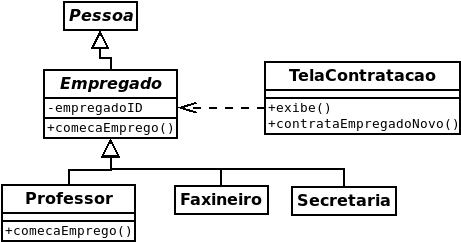
\includegraphics[scale=0.65]{uniRH.png}
\end{center}
\caption{Implementação parcial do sistema de recursos humanos da universidade.} \label{fig:uniRH}
\end{figure}

Considere um exemplo um pouco mais realístico de polimorfismo explorando o projeto de como a universidade lida com a contratação de pessoal modelada na figura \ref{fig:uniRH}. Há uma maneira padrão para a universidade contratar pessoal: Uma vez contratada uma pessoa, ela é incluída no plano de saúde da universidade e ganha um crachá. Quando um professor é contratado, o mesmo processo é seguido, mas, além disso, uma vaga de estacionamento é atribuída para o novo professor se houver vaga disponível, senão ele entra na fila de espera por vagas de estacionamento.

Se o método \emph{comecaEmprego()} for implementado na classe \emph{Empregado}, ele implementa o comportamento necessário para adicionar uma pessoa ao plano de saúde da universidade e a geração do crachá. O método \emph{comecaEmprego()} na classe \emph{Professor} terá de ser sobrescrito. Ele chama o método da classe \emph{Empregado}, pois professores também são inclusos no plano de saúde da universidade e recebem crachás, mas, além disso, reserva uma vaga de estacionamento.

Por ser capaz de enviar a mensagem \emph{comecaEmprego()} para qualquer tipo de empregado, não há a necessidade de usar complicadas instruções condicionais no método \emph{contrataEmpregadoNovo()} do objeto tela. Este método não precisa mandar uma mensagem \emph{comecaProfessor()} para objetos professores, \emph{comecaFaxineiro()} para objetos faxineiros, etc. Ele só precisa enviar \emph{comecaEmprego()} para qualquer tipo de empregado e o objeto fará a coisa certa. Como resultado, você pode acrescentar novos tipos de empregados (como o \emph{Administrativo}) e não precisa mudar o objeto tela. Isto também significa que a classe \emph{TelaContratacao} é fracamente acoplada à hierarquia de classes, o que permite a extensão do sistema facilmente.

É importante mencionar que o projeto da figura \ref{fig:uniRH} não é um muito bom. Uma maneira melhor de fazer é refatorar a hierárquica usando o padrão de projeto \emph{Papéis interpretados} ilustrado na figura \ref{fig:uniRH2}. Este padrão separa o conceito de alguém ser uma pessoa e o papel que ela interpreta no trabalho. Esta separação permite que uma pessoa interprete mais de um papel no trabalho.

\begin{figure}
\begin{center}
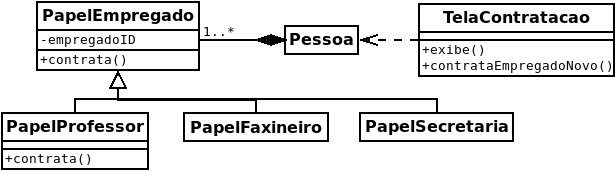
\includegraphics[scale=0.65]{uniRH2.png}
\end{center}
\caption{Sistema de recursos humanos da universidade refatorado.} \label{fig:uniRH2}
\end{figure}

\section{Interfaces}

Uma interface é a definição de uma coleção de um ou mais métodos e zero ou mais atributos. Interfaces idealmente definem um conjunto de comportamentos coesos. Interfaces são implementadas por classes e componentes. Para implementar uma interface, uma classe ou componente deve incluir os métodos definidos pela interface. Por exemplo, a figura \ref{fig:ifcUml} ilustra que a classe \emph{Estudante} implementa as interfaces \emph{Serializavel}\footnote{Observe que estamos traduzindo \emph{Serializable} por Serializavel, embora não achemos que este termo reflita adequadamente a noção do que esta interface permite que seja feito com os objetos que a implementam. A ideia é que um objeto serializável é um objeto que pode ser convertido para um formato textual que permita a  transmissão do objeto serializado através da rede para um processo remoto ou local. O objeto serializado também pode ser armazenado em uma memória permanente e recuperado depois.} e \emph{Buscavel}. Para implementar a interface \emph{Buscavel}, \emph{Estudante} deve definir o método \emph{busca()} com o parâmetro \emph{critério}. Qualquer classe ou componente pode implementar zero ou mais interfaces e uma ou mais classes podem implementar qualquer interface. Interfaces são usadas para promover a consistência dentro de seus modelos e código fonte.

\begin{figure}[h]
\begin{center}
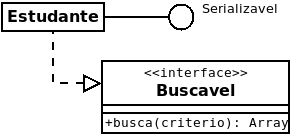
\includegraphics[scale=0.7]{ifcUml.png}
\end{center}
\caption{As duas notações para interfaces em UML.} \label{fig:ifcUml}
\end{figure}

Interfaces servem para garantir acoplamentos fracos. Eles permitem a uma classe participar de um conjunto comum de funcionalidades sem que nenhuma outra classe tenha que saber algo mais além dela implementar a interface. Um objeto GUI, por exemplo, pode exibir uma lista de estudantes que atendem um critério de busca sem conhecer nada da classe \emph{Estudante}, exceto que ela implementa a interface \emph{Buscavel} e a interface \emph{Descrição} que tem um método que apresenta o estudante. A mesma GUI pode ser usada para realizar a mesma ação com os professores, se a classe \emph{Professor} também implementar estas duas interfaces. De modo análogo, se a classe \emph{Disciplina} também implementar estas interfaces, a GUI também pode ser usada para exibir uma lista de disciplinas que atendam ao critério de busca. A GUI não precisa saber nada sobre a classe, só que ela implementa as interfaces. Isto mostra um fraco acoplamento entre a GUI e os objetos das classes que ela exibe.

Em linguagens como Java e C\#, interfaces fazem parte do mecanismo de tipagem. Isto é, a classe \emph{Estudante} da figura \ref{fig:ifcUml} tem pelo menos três tipos: \emph{Estudante}, \emph{Serializavel} e \emph{Buscavel}. Ela também tem o tipo de todas as suas superclasses. Por exemplo, se \emph{Estudante} herda de \emph{Pessoa} e ela implementa a interface \emph{Printable}, então os objetos estudantes também são do tipo \emph{Pessoa} e \emph{Printable}. O mecanismo de tipo da sua linguagem de implementação afetará a extensão do polimorfismo suportado.

A figura \ref{fig:ifcUml} mostra ainda que existem duas notações em UML para indicar que algo implementa uma interface: A notação da circunferência com linha contínua (vulgarmente chamada de pirulito) da interface \emph{Serializavel} e a notação em caixa usada para a interface \emph{Buscavel}. A primeira tem a vantagem de ser mais compacta, enquanto a segunda fornece mais detalhes. A caixa da interface \emph{Buscavel} é a mesma da classe com o estereótipo \emph{interface}. Estereótipo é um mecanismo para definir extensões comuns e consistentes na notação UML. A seta tracejada de \emph{Estudante} para \emph{Buscavel} é uma relação \emph{realiza} em UML. Isto significa que \emph{Estudante} implementa (realiza) a interface \emph{Buscavel}.

\section{Componentes}

Um componente é uma unidade modular, extensível de distribuição independente que tem interface(s) contratualmente especificadas e dependências explicitamente definidas, se houver. Idealmente, componentes devem ser modulares, extensíveis e abertas. Modularidade implica em que um componente contém tudo que ele precisa para cumprir suas responsabilidades. Extensibilidade implica em que um componente pode ser melhorado para cumprir outras responsabilidades além daquelas para as quais foi originalmente projetada. E aberta implica que ele possa funcionar em várias plataformas e interagir com outros componentes através de uma única interface de programação.

Componentes, como classes, implementam interfaces. As interfaces de um componente definem os seus pontos de acesso. Componentes são tipicamente implementadas como coleções de classes, idealmente, classes que formam um subconjunto coeso dos seus sistemas completos. Componentes são tipicamente pesados e podem até ser pensados como classes grandes ou mesmo subsistemas. Por exemplo, um banco de dados pode ser um componente, ou uma coleção de classes de negócio/domínio que implementam os comportamentos requeridos pelas pessoas dentro da sua aplicação pode ser um componente.

Diagramas de Componentes mostram os componentes de software que compõem um pedaço maior de software, suas interfaces e suas inter-relações. Vamos considerar um componente como sendo um item grande usado nas operações diárias do seu negócio -- por exemplo, um subsistema comum, um sistema comercial padrão (COTS - commercial off-the-self system), uma aplicação OO ou uma aplicação antiga empacotada. De muitas maneiras, um diagrama de componentes é simplesmente um diagrama de classes numa escala maior, apenas menos detalhada.

A figura \ref{fig:compo} mostra um exemplo de um diagrama de componente usado para modelar uma arquitetura de negócio para a universidade. As caixas representam componentes -- neste caso, as interfaces de usuário que o pessoal usa para interagir com os sistemas da universidade, os componentes de negócio tais como \emph{Instalacoes} ou componentes técnicos como o componente de \emph{Seguranca} ou banco de dados.

\begin{figure}
\begin{center}
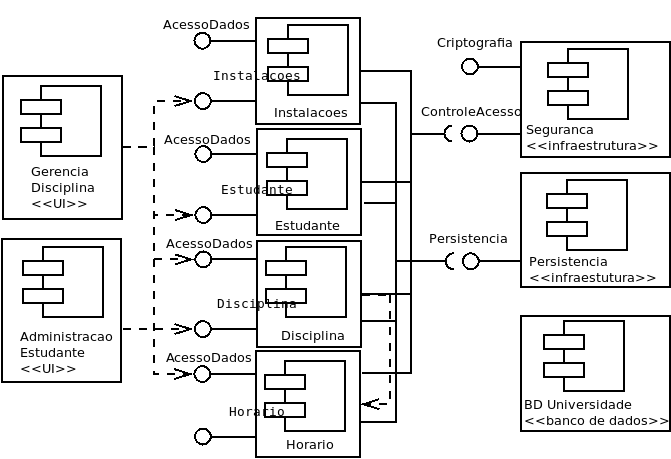
\includegraphics[scale=0.5]{componente.png}
\end{center}
\caption{Diagrama de componentes da UML 2.} \label{fig:compo}
\end{figure}

Na figura \ref{fig:compo}, você pode observar que os componentes UI (interface usuário) têm dependências nas interfaces dos componentes de negócio. Ao fazer os componentes UI dependentes das interfaces e não dos próprios componentes, você torna possível substituir os componentes com diferentes implementações desde que eles implementem as interfaces dadas. Isto reduz acoplamento. De modo similar, é possível que os componentes de negócio dependam uns dos outros. Por exemplo, o componente \emph{Disciplina} é acoplado ao componente \emph{Horario}. 

Uma notação interessante da UML 2 é o soquete. Um soquete é o semicírculo em torno do símbolo pirulito, como pode ser visto com as interfaces \emph{ControleAcesso} e \emph{Persistencia} com as componentes de \emph{Seguranca} e \emph{Persistencia}, respectivamente. Este símbolo é usado para indicar que alguma coisa requer a existência de uma interface. Por exemplo, as quatro componentes de negócios (\emph{Instalacoes}, \emph{Estudante}, \emph{Disciplina} e \emph{Horario}) todas requerem a existência de alguma coisa que implemente a interface \emph{ControleAcesso}.

Observe a consistência da notação entre diagramas de classes e diagramas de componentes. Ambos usam exatamente a mesma notação para relacionamentos de dependência, vide figura \ref{fig:clsDep}. Esta é uma característica boa da UML: A notação é consistente. Existem uns poucos detalhes da UML que não são consistentes, mas, na maioria dos casos, cada conceito é modelado da mesma maneira através dos diferentes diagramas.

\section{Padrões}

Com a prática, você vai sentir que você repetidamente está resolvendo os mesmos problemas. Se você não resolveu pessoalmente um certo problema, é muito provável que alguém ou resolveu este problema, ou um muito similar. O problema em que você está trabalhando pode ser simples ou complexo, mas, geralmente, já foi trabalhado antes. Não seria bom ser capaz de encontrar uma solução facilmente, ou, pelo menos, uma solução parcial, para o problema? Pense em quanto tempo e esforço poderiam ser poupados se você tivesse acesso a uma biblioteca de soluções para problemas de desenvolvimento de sistemas comuns. É disto que tratam os padrões (\textit{patterns}).

Um padrão é uma solução para um \emph{problema comum} levando em conta as forças relevantes, apoiando efetivamente o reuso de técnicas e procedimentos comprovados de outros desenvolvedores. Existem diferentes tipos de \emph{padrões}, incluindo \emph{padrões de análise}, \emph{padrões de projeto} e \emph{padrões de processos}. Padrões de análise descrevem uma solução para problemas comuns encontrados na análise da lógica de negócios/domínio de uma aplicação, padrões de projeto descrevem uma solução para problemas comuns encontrados no projeto de sistemas e padrões de processos se aplicam a questões de processos de software. O livro \cite{design:patterns} é a referência de base clássica que popularizou o uso de padrões em software.

Por exemplo, é comum descobrir classes em sua aplicação que devem ter apenas uma instância. Por exemplo, deve haver apenas uma janela de edição para um dado tipo de alteração, ou alguma informação de configuração só pode ser armazenada num único local, ou você precisa manter valores constantes num único lugar. Nestes casos todos, você precisa de uma única instância da classe em questão -- uma única instância de uma caixa de diálogo, uma única instância da informação de configuração e uma única instância das constantes. Este problema é resolvido pelo padrão \emph{Singleton}\label{p:singleton}, um padrão de projeto que mostra como apenas uma instância de uma classe pode existir. A figura \ref{fig:singleton} mostra o diagrama de classe de um \emph{Singleton}. Um atributo estático existe para acessar a instância única, se ela existe. O método \emph{create()}, talvez melhor chamado de \emph{getSingleton()}, permite acessá-lo e criá-lo se necessário. \emph{Singleton} é um padrão simples e muito usado.

\begin{figure}
\begin{center}
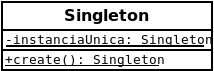
\includegraphics[scale=0.7]{singleton.png}
\end{center}
\caption{Padrão de projeto \emph{Singleton}} \label{fig:singleton}
\end{figure}

Existem padrões muito complexos. A maioria dos padrões são baseados em três ou mais classes. O principal desafio com os padrões é que quando você aprende sobre eles, tudo parece ser um padrão e, às vezes, isto é verdade. O perigo é que você pode exagerar na construção do seu software, aumentando a dificuldade de manutenção, apesar de reduzir o tempo para implementar os requisitos. Para evitar, atenuar, este problema, o modelamento ágil (AM) inclui a prática de \emph{aplicar gentilmente os padrões}, onde você introduz os padrões pela \emph{refatoração} do seu projeto lentamente no lugar de aplicá-los quando você acha que precisa deles.
\cite{DP:explained} considera que um bom momento para aprender padrões de projeto é quando se está aprendendo projetos com orientação a objetos.

\section{O que foi aprendido}

Neste capítulo, você foi apresentado aos principais conceitos do paradigma da orientação objeto e à notação básica da UML 2 para modelar alguns destes conceitos. Os conceitos de OO são numerosos e, às vezes, complexos. Não se preocupe, é normal se sentir sobrecarregado no início, mas com a prática você passa a dominá-los. 

\section{Questões de Revisão}

\begin{enumerate}
\item Discorra sobre a diferença entre herança e composição. Quais são as vantagens e desvantagens de cada um deles. Você pode implementar um com o outro?

\item Como uma classe se assemelha com uma tabela de banco de dados? Como elas se diferem? Como estas diferenças e similaridades justificam modelos de classes e modelos de dados?

\item Discorra sobre a diferença entre associação e composição. Quais são as vantagens e desvantagens de cada um?

\item Quando você deve aplicar herança? Quando não? Forneça exemplos de quando herança é apropriada e quando não é.

\item Compare e oponha os conceitos de acoplamento e coesão. Como eles se relacionam, se é que se relacionam?

\item Descreva o relacionamento entre o polimorfismo e a tipagem.

\item Através da Internet, pesquise sobre tecnologias de bancos dedados, incluindo bancos de dados relacionais, bancos de dados de objetos, bancos de dados relacionais-objetos, bancos de dados XML, bancos de dados hierárquicos e bancos de dados em redes. Forneça pelo menos um exemplo de cada. Compare as tecnologias, listando as vantagens, desvantagens e uma indicação de quando você deve usar cada um.

\item Como interfaces reduzem o acoplamento de sistemas OO? Como elas podem aumentar? Por que?
\end{enumerate}
